%% abtex2-modelo-trabalho-academico.tex, v-1.9.2 laurocesar
%% Copyright 2012-2017 by abnTeX2 group at http://abntex2.googlecode.com/ 
%%
%% This work may be distributed and/or modified under the
%% conditions of the LaTeX Project Public License, either version 1.3
%% of this license or (at your option) any later version.
%% The latest version of this license is in
%%   http://www.latex-project.org/lppl.txt
%% and version 1.3 or later is part of all distributions of LaTeX
%% version 2005/12/01 or later.
%%
%% This work has the LPPL maintenance status `maintained'.
%% 
%% The Current Maintainer of this work is Emílio Eiji Kavamura,
%% eek.edu@outlook.com; emilio.kavamura@ufpr.br
%% Further information about abnTeX2 are available on 
%%
%% http://abntex2.googlecode.com/
%%
%% https://code.google.com/p/abntex2/issues/ 
%%
%% Further information about UFPR abnTeX2 are available on 
%%
%% https://github.com/eekBR/ufpr-abntex/
%%
%% This work consists of the files 
% 
%          main.tex   programa principal
%      00-dados.tex   entrada de dados 
%    00-pacotes.tex   pacotes carregados no modelo
% 00-pretextual.tex   processamento dos elementos pre-textuais
%          UFPR.sty   ajusta do modelo canonico às normas  UFPR
%
%    referencias.bib
%                     e outras arquivos de imagens
%
%
%------------------------------------------------------------------------
% ------------------------------------------------------------------------
% abnTeX2: Modelo de Trabalho Academico (tese de doutorado, dissertacao de
% mestrado e trabalhos monograficos em geral) em conformidade com 
% ABNT NBR 6023:2018: Informação e documentação - Referências - Elaboração
% ------------------------------------------------------------------------
% ------------------------------------------------------------------------
%
% DATA DE ATUALIZAÇÃO: 2020-06-10

\documentclass[
        % -- opções da classe memoir --
        12pt,                           % tamanho da fonte
        openright,                      % capítulos começam em pág ímpar (insere página vazia caso preciso)
        %twoside,                        % para impressão em verso e anverso. Oposto a oneside
        oneside,
        a4paper,                        % tamanho do papel. 
        % -- opções da classe abntex2 --
        chapter=TITLE,         % títulos de capítulos convertidos em letras maiúsculas
        section=TITLE,         % títulos de seções convertidos em letras maiúsculas
        subsection=Title,      % títulos de subseções convertidos em letras maiúsculas
        %subsubsection=TITLE,  % títulos de subsubseções convertidos em letras maiúsculas
        % -- opções do pacote babel --
        english,                        % idioma adicional para hifenização
        %french,                         % idioma adicional para hifenização
        spanish,                        % idioma adicional para hifenização
        portugues,                      % o último idioma é o principal do documento
        %%%%%%%%%%%%
        %eek: colocação da opção para o sumario ter formatação tradicional
        sumario=tradicional             % título no formato tradicional
        ]{abntex2}


\usepackage{UFPR}
% Pacotes básicos 
% ----------------------------------------------------------
%\usepackage{lmodern}			% Usa a fonte Latin Modern			
\usepackage[T1]{fontenc}		% Selecao de codigos de fonte.
\usepackage[utf8]{inputenc}		% Codificacao do documento (conversão automática dos acentos)
\usepackage{lastpage}			% Usado pela Ficha catalográfica
\usepackage{indentfirst}		% Indenta o primeiro parágrafo de cada seção.
\usepackage{color}		    	% Controle das cores
\usepackage{graphicx}			% Inclusão de gráficos
\usepackage{microtype} 			% para melhorias de justificação
\usepackage{ifthen}		    	% para montar condicionais
\usepackage[brazil]{babel}		% para utilizar termos em portugues
\usepackage[final]{pdfpages}    % para incluir páginas de arquivos pdf
\usepackage{lipsum}				% para geração de dummy text
\usepackage{csquotes}

%\usepackage[style=long]{glossaries}
%\usepackage{abntex2glossaries}


\usepackage{cancel} 		% permite representar o cancelamento de termos em texto ou equacoes	
\usepackage{xcolor} 		% cores extendidas	
\usepackage{smartdiagram}   	% gera diagramas a partir de listas
%\usepackage{float} 		% Para a figura ficar na posição correta	    
\usepackage{textcomp} 		% supporte para fontes da Text Companion 
\usepackage{longtable}		% uso de longtable
\usepackage{amsmath}		% simbolos matematicos
\usepackage{lscape}		% páginas em paisagem
\usepackage{multicol}		% mescla de colunas em tabelas
\usepackage{multirow}		% mescla de linhas em tabelas
\usepackage{newfloat} 		% criação do indice de quadros
%\usepackage{caption} 		% configura legenda 
	%[format=plain]
	%\renewcommand\caption[1]{%
    	%\captionsetup{font=small}	% tamanho da fonte 10pt
    	%,format=hang
 	% \caption{#1}}
	%\captionsetup{width=0.8\textwidth}
\captiondelim{-- }
\captiontitlefont{\small}
\captionnamefont{\small}

% Pacotes de citações BibLaTeX
% ----------------------------------------------------------
\usepackage[style=abnt,
	backref=true,
	repeatfields=true, 
	backend=biber,
	citecounter=true,
	backrefstyle=three, 
	url=true]{biblatex}

% Texto padrão para as referências
% ----------------------------------------------------------
\DefineBibliographyStrings{brazil}{%
	 backrefpage  = {Citado \arabic{citecounter} vez na página},		% originally "cited on page"
	 backrefpages = {Citado \arabic{citecounter} vezes nas páginas},	% originally "cited on pages"
	 urlfrom      = {Dispon\'ivel em},
}

% Ajusta indentação de Referencias no ToC
% ----------------------------------------------------------
\defbibheading{bay}[\bibname]{%
  \chapter*{#1}%
  \markboth{#1}{#1}%
  \addcontentsline{toc}{chapter}
  {\protect\numberline{}\bibname}
}

% Formatando o avançao dos títulos no sumário 
% ----------------------------------------------------------
\makeatletter
	\pretocmd{\chapter}{\addtocontents{toc}{\protect\addvspace{-12\p@}}}{}{}
	\pretocmd{\section}{\addtocontents{toc}{\protect\addvspace{-3\p@}}}{}{}
\makeatother

% Para retirar os símbolos <> da URL  
% ----------------------------------------------------------
\DeclareFieldFormat{illustrated}{\addspace #1\isdot}%
%\DeclareFieldFormat{url}{\bibstring{urlform}\addcolon\addspace<\url{#1}>}%
%\DeclareFieldFormat{url}{\bibstring{urlfrom}\addcolon\addspace<\url{#1}>}%
\DeclareFieldFormat{url}{\bibstring{urlfrom}\addcolon \space\addspace{#1}} 
% remove <> em urls de acordo com abnt-6023:2018	

% Ajustar o espaço para a formatação da data
% ----------------------------------------------------------
\DeclareFieldFormat{urldate}{\bibstring{urlseen}\addcolon\addspace #1}%
\DeclareFieldFormat*{note}{\addspace #1}%

% Para ajustar o tamanho da fonte do número da primeira página do capítulo
% comando utilizado na parte textual 
% ----------------------------------------------------------
\makepagestyle{chapfirst}% Just for the first page of a chapter
\makeoddhead{chapfirst}{}{}{\normalsize{\thepage}}

% Define a formatação dos capítulos póstextuais numerados
% ----------------------------------------------------------
\newcommand{\poschap}[1]{
	\stepcounter{chapter}
	\markboth{#1}{#1}%
	\pdfbookmark[2]{#1}{#1}
	\addtocontents{toc}{\vspace{-0pt}}
	\addcontentsline{toc}{chapter}{\hspace{14.5mm}\textbf{\appendixname~
	\thechapter~- #1}}
	\chapter*{\appendixname\space\space\thechapter~- \uppercase{#1}}%
	{}
}
\newcommand{\refap}[1]{\hyperref[#1]{Apêndice~\ref{#1}}} 	% Referência apÊndices
% uso do tikz e pgfplots
% ----------------------------------------------------------
%\usetikzlibrary{external}
\usetikzlibrary{arrows,calc,patterns,angles,quotes}
\usepackage{pgfplots}
\pgfplotsset{compat=1.15}



%%%%%%%%%%%%%%%%%%%%%%%%%%%%%%%%%%%%%%%%%%%%%%%%%%%%%%%
% Arquivo para entrada de dados para a parte pré textual
%%%%%%%%%%%%%%%%%%%%%%%%%%%%%%%%%%%%%%%%%%%%%%%%%%%%%%%
% 
% Basta digitar as informações indicidas, no formato 
% apresentado.
%
%%%%%%%
% Os dados solicitados são, na ordem:
%
% título do trabalho
% nome do autor
% local 
% data (ano com 4 dígitos)
% orientador
% coorientador
% instituição
% tipo de trabalho
% preambulo
% epígrafe
% resumo
% palavras chave
% abstract
% keywords
% agradecimentos
% dedicatoria
% siglas 
% simbolos
%
%%%%%%%%%%%%%%%%%%%%%%%%%%%%%%%%%%%%%%%%%%%%%%%%%%%%%%%
% ---
% Informações de dados para CAPA e FOLHA DE ROSTO
% ---
\titulo{\textbf{Modelo de\\ trabalho acadêmico com \abnTeX}}
\autor{Rodrigo H M}
\local{Curitiba}
\data{2015} %Apenas ano 4 dígitos

% Orientador ou Orientadora
\orientador{Prof Emílio Eiji Kavamura, MSc}
\orientadora{}%Prof\textordfeminine Grace Kelly, DSc}

% Coorientador ou Coorientadora
\coorientador{}%Prof Morgan Freeman, DSc}
\coorientadora{Prof\textordfeminine Audrey Hepburn, DEng}

% Segundo Coorientador ou Segunda Coorientadora
\scoorientador{Prof Jack Nicholson, DEng}
\scoorientadora{}%Prof\textordfeminine Ingrid Bergman, DEng}

\instituicao{%
  Universidade Federal do Paraná
  }
  %\par
  %Departamento de Expressão Gráfica
  %\par
  %Curso de Expressão Gráfica}
\tipotrabalho{Trabalho Acadêmico}
% O preambulo deve conter o tipo do trabalho, o objetivo, 
% o nome da instituição e a área de concentração 
\preambulo{Trabalho apresentado como requisito parcial para a obtenção do grau de Bacharel em Expressão Gráfica no curso de Expressão Gráfica, Setor de Exatas da Universidade Federal do Paraná.}

\newcommand{\imprimirCurso}
{Programa de P\'os Gradua\c{c}\~ao em Engenharia da Constru\c{c}\~ao Civil}

\newcommand{\imprimirDataDefesa}{
09 de Dezembro de 2018}
% ---

% ---
\newcommand{
\FichaCatalografica}{%\color{blue}

\imprimirautor
	
	\hspace{0.5cm} \imprimirtitulo  / \imprimirautor. --
	\imprimirlocal, \imprimirdata-
	
	\hspace{0.5cm} \pageref{LastPage} p. : il. (algumas color.) ; 30 cm.\\
	
	\hspace{0.5cm} \imprimirorientadorRotulo~\imprimirorientador\\
	
	\hspace{0.5cm}
	\parbox[t]{\textwidth}{\imprimirtipotrabalho~--~\imprimirinstituicao,
	\imprimirdata.}\\
	
	\hspace{0.5cm}
	   \begin{minipage}{.70\textwidth}
	    	1. \PalavraschaveTexto
		
		I. \imprimirorientador.
		
		II. \imprimirinstituicao.
		
		III. \imprimirCurso
		
		IV. \imprimirtitulo\\ 			
	
	\hspace{8.75cm} CDU 02:141:005.7\\
	\end{minipage}
	}

% ---
\newcommand{
\AssinaAprovacao}{

\assinatura{%\textbf
   {Professor} \\ Convidado 1}
   \assinatura{%\textbf
   {Professor} \\ Convidado 2}
   \assinatura{%\textbf
   {Professor} \\ Convidado 3}
   %\assinatura{%\textbf{Professor} \\ Convidado 4}
      
   \begin{center}
    \vspace*{0.5cm}
    %{\large\imprimirlocal}
    %\par
    %{\large\imprimirdata}
    \imprimirlocal, \imprimirDataDefesa.
    \vspace*{1cm}
  \end{center}
  }
  
% ---
\newcommand{
\Errata}{%\color{blue}
Elemento opcional da \citeonline[4.2.1.2]{NBR14724:2011}. Exemplo:

\vspace{\onelineskip}

FERRIGNO, C. R. A. \textbf{Tratamento de neoplasias ósseas apendiculares com
reimplantação de enxerto ósseo autólogo autoclavado associado ao plasma
rico em plaquetas}: estudo crítico na cirurgia de preservação de membro em
cães. 2011. 128 f. Tese (Livre-Docência) - Faculdade de Medicina Veterinária e
Zootecnia, Universidade de São Paulo, São Paulo, 2011.

\begin{table}[htb]
\center
\footnotesize
\begin{tabular}{|p{1.4cm}|p{1cm}|p{3cm}|p{3cm}|}
  \hline
   \textbf{Folha} & \textbf{Linha}  & \textbf{Onde se lê}  & \textbf{Leia-se}  \\
    \hline
    1 & 10 & auto-conclavo & autoconclavo\\
   \hline
\end{tabular}
\end{table}
}

% ---
\newcommand{
\EpigrafeTexto}{%\color{blue}
\textit{``Não vos amoldeis às estruturas deste mundo, \\
		mas transformai-vos pela renovação da mente, \\
		a fim de distinguir qual é a vontade de Deus: \\
		o que é bom, o que Lhe é agradável, o que é perfeito.\\
		(Bíblia Sagrada, Romanos 12, 2)}
}
% ---
\newcommand{
\ResumoTexto}{%\color{blue}
Segundo a \citeonline[3.1-3.2]{abntex2modelo}, o resumo deve ressaltar o  objetivo, o método, os resultados e as conclusões do documento. A ordem e a extensão destes itens dependem do tipo de resumo (informativo ou indicativo) e do tratamento que cada item recebe no documento original. O resumo deve ser precedido da referência do documento, com exceção do resumo inserido no próprio documento. (\ldots) As palavras-chave devem figurar logo abaixo do  resumo, antecedidas da expressão Palavras-chave:, separadas entre si por ponto e finalizadas também por ponto.
}
% ---
\newcommand{
\PalavraschaveTexto}{%\color{blue}
latex. abntex. editoração de texto.
}
% ---
\newcommand{
\AbstractTexto}{%\color{blue}
This is the english abstract.
}
% ---
\newcommand{
\KeywordsTexto}{%\color{blue}
latex. abntex. text editoration.
}
% ---
\newcommand{
\AgradecimentosTexto}{%\color{blue}
Os agradecimentos principais são direcionados à Gerald Weber, Miguel Frasson, Leslie H. Watter, Bruno Parente Lima, Flávio de  Vasconcellos Corrêa, Otavio Real Salvador, Renato Machnievscz\footnote{Os nomes dos integrantes do primeiro
projeto abn\TeX\ foram extraídos de \url{http://codigolivre.org.br/projects/abntex/}} e todos aqueles que contribuíram para que a produção de trabalhos acadêmicos conforme as normas ABNT com \LaTeX\ fosse possível.

Agradecimentos especiais são direcionados ao Centro de Pesquisa em Arquitetura da Informação\footnote{\url{http://www.cpai.unb.br/}} da Universidade de Brasília (CPAI), ao grupo de usuários
\emph{latex-br}\footnote{\url{http://groups.google.com/group/latex-br}} e aos novos voluntários do grupo \emph{\abnTeX}\footnote{\url{http://groups.google.com/group/abntex2} e
\url{http://abntex2.googlecode.com/}}~que contribuíram e que ainda
contribuirão para a evolução do \abnTeX.

Os agradecimentos principais são direcionados à Gerald Weber, Miguel Frasson, Leslie H. Watter, Bruno Parente Lima, Flávio de Vasconcellos Corrêa, Otavio Real Salvador, Renato Machnievscz\footnote{Os nomes dos integrantes do primeiro
projeto abn\TeX\ foram extraídos de \url{http://codigolivre.org.br/projects/abntex/}} e todos aqueles que contribuíram para que a produção de trabalhos acadêmicos conforme as normas ABNT com \LaTeX\ fosse possível.
}
% ---
\newcommand{
\DedicatoriaTexto}{%\color{blue}
\textit{ Este trabalho é dedicado às crianças adultas que,\\
   quando pequenas, sonharam em se tornar cientistas.}
	}
% ---	


% compila o indice
% ----------------------------------------------------------

\makeindex
% ----------------------------------------------------------
% Início do documento
% ----------------------------------------------------------
\begin{document}
% ----------------------------------------------------------
% Adequando o uppercase titulo dos elementos nas suas respectivas legendas
% Definicoes que n\~ao funcionaram quando colocados no arquivo de estilos ou de pacotes

\renewcommand{\bibname}{{REFER\^ENCIAS}}
\renewcommand{\tablename}{TABELA }
\renewcommand{\figurename}{FIGURA }
\renewcommand{\figureautorefname}{FIGURA}
\renewcommand{\tableautorefname}{TABELA}
\newcommand{\equationname}{EQUA\c{C}\~AO~}
\renewcommand{\equationautorefname}{EQUA\c{C}\~AO~}

% Para ajustar o tamanho da fonte do número da primeira página do capítulo
\aliaspagestyle{chapter}{chapfirst}% customizing chapter pagestyle

% ----------------------------------------------------------
% ELEMENTOS PRÉ-TEXTUAIS
% ----------------------------------------------------------
 %\pretextual

% ---
% Capa
% ---
\imprimircapa
% ---

% ---
% Folha de rosto
% (o * indica que haverá a ficha bibliográfica)
% ---
\imprimirfolhaderosto*
% ---

% ---
% Inserir a ficha bibliografica
% ---

% Isto é um exemplo de Ficha Catalográfica, ou ``Dados internacionais de
% catalogação-na-publicação''. Você pode utilizar este modelo como referência. 
% Porém, provavelmente a biblioteca da sua universidade lhe fornecerá um PDF
% com a ficha catalográfica definitiva após a defesa do trabalho. Quando estiver
% com o documento, salve-o como PDF no diretório do seu projeto e substitua todo
% o conteúdo de implementação deste arquivo pelo comando abaixo:
%
% \begin{fichacatalografica}
%     \includepdf{fig_ficha_catalografica.pdf}
% \end{fichacatalografica}
\begin{fichacatalografica}%\color{blue}
	\vspace*{\fill}					% Posição vertical
	\hrule							% Linha horizontal
	\begin{center}					% Minipage Centralizado
	\begin{minipage}[c]{12.5cm}		% Largura
	
	\imprimirautor
	
	\hspace{0.5cm} \imprimirtitulo  / \imprimirautor. --
	\imprimirlocal, \imprimirdata-
	
	\hspace{0.5cm} \pageref{LastPage} p. : il. (algumas color.) ; 30 cm.\\
	
	\hspace{0.5cm} \imprimirorientadorRotulo~\imprimirorientador\\
	
	\hspace{0.5cm}
	\parbox[t]{\textwidth}{\imprimirtipotrabalho~--~\imprimirinstituicao,
	\imprimirdata.}\\
	
	\hspace{0.5cm}
		1. Palavra-chave1.
		2. Palavra-chave2.
		I. \imprimirorientador.
		II. \imprimirinstituicao.
		III. Faculdade de xxx.
		IV. Título\\ 			
	
	\hspace{8.75cm} CDU 02:141:005.7\\
	
	\end{minipage}
	\end{center}
	\hrule
\end{fichacatalografica}
% ---

% ---
% Inserir errata
% ---
\begin{errata}%\color{blue}
Elemento opcional da \citeonline[4.2.1.2]{NBR14724:2011}. Exemplo:

\vspace{\onelineskip}

FERRIGNO, C. R. A. \textbf{Tratamento de neoplasias ósseas apendiculares com
reimplantação de enxerto ósseo autólogo autoclavado associado ao plasma
rico em plaquetas}: estudo crítico na cirurgia de preservação de membro em
cães. 2011. 128 f. Tese (Livre-Docência) - Faculdade de Medicina Veterinária e
Zootecnia, Universidade de São Paulo, São Paulo, 2011.

\begin{table}[htb]
\center
\footnotesize
\begin{tabular}{|p{1.4cm}|p{1cm}|p{3cm}|p{3cm}|}
  \hline
   \textbf{Folha} & \textbf{Linha}  & \textbf{Onde se lê}  & \textbf{Leia-se}  \\
    \hline
    1 & 10 & auto-conclavo & autoconclavo\\
   \hline
\end{tabular}
\end{table}

\end{errata}
% ---

% ---
% Inserir folha de aprovação
% ---

% Isto é um exemplo de Folha de aprovação, elemento obrigatório da NBR
% 14724/2011 (seção 4.2.1.3). Você pode utilizar este modelo até a aprovação
% do trabalho. Após isso, substitua todo o conteúdo deste arquivo por uma
% imagem da página assinada pela banca com o comando abaixo:
%
% \includepdf{folhadeaprovacao_final.pdf}
%
\begin{folhadeaprovacao}%\color{blue}

  \begin{center}
    {\ABNTEXchapterfont
    {\bfseries\folhadeaprovacaoname}\par\phantom{}\par
    %\large
    \MakeUppercase\imprimirautor}

    \vspace*{\fill}\vspace*{\fill}
    \begin{center}
      \ABNTEXchapterfont
      %\bfseries\Large
      \MakeUppercase\imprimirtitulo
    \end{center}
    \vspace*{\fill}
    
    \hspace{.45\textwidth}
    %\begin{minipage}{.5\textwidth}
        \imprimirpreambulo, pela seguinte banca examinadora:
    %\end{minipage}%
    \vspace*{\fill}
   \end{center}
       \assinatura{\textbf{\imprimirorientador} \\ Orientador} 
   \assinatura{%\textbf
   {Professor} \\ Convidado 1}
   \assinatura{%\textbf
   {Professor} \\ Convidado 2}
   \assinatura{%\textbf
   {Professor} \\ Convidado 3}
   %\assinatura{%\textbf{Professor} \\ Convidado 4}
      
   \begin{center}
    \vspace*{0.5cm}
    %{\large\imprimirlocal}
    %\par
    %{\large\imprimirdata}
    \imprimirlocal, 24 de novembro de 2012.
    \vspace*{1cm}
  \end{center}
  
\end{folhadeaprovacao}
% ---

% ---
% Dedicatória
% ---
\begin{dedicatoria}
   \vspace*{\fill}
   \centering
   \noindent
   \DedicatoriaTexto
    \vspace*{\fill}
\end{dedicatoria}
% ---

% ---
% Agradecimentos
% ---
\begin{agradecimentos}
\AgradecimentosTexto
\end{agradecimentos}
% ---

% ---
% Epígrafe
% ---
\begin{epigrafe}
    \vspace*{\fill}
	\begin{flushright}
        \EpigrafeTexto
	\end{flushright}
\end{epigrafe}
% ---

% ---
% RESUMOS
% ---

% resumo em português
\setlength{\absparsep}{18pt} % ajusta o espaçamento dos parágrafos do resumo
\begin{resumo}
    \ResumoTexto
    \vspace{\onelineskip}
    \noindent 
    \textbf{Palavras-chaves}: \PalavraschaveTexto
\end{resumo}

% resumo em inglês
\begin{resumo}[ABSTRACT]
 \begin{otherlanguage*}{english}
   \AbstractTexto
   \vspace{\onelineskip}
 
   \noindent 
   \textbf{Key-words}: \KeywordsTexto
 \end{otherlanguage*}
\end{resumo}

% resumo em francês 
% \begin{resumo}[RESUME]%Résumé
%  \begin{otherlanguage*}{french}
%     Il s'agit d'un résumé en français.
%  
%    \textbf{Mots-clés}: latex. abntex. publication de textes.
%  \end{otherlanguage*}
% \end{resumo}
% 
% % resumo em espanhol
% \begin{resumo}[RESUMEN]
%  \begin{otherlanguage*}{spanish}
%    Este es el resumen en español.
%   
%    \textbf{Palabras clave}: latex. abntex. publicación de textos.
%  \end{otherlanguage*}
% \end{resumo}
% ---

% ---
% inserir lista de ilustrações
% ---
\pdfbookmark[0]{\listfigurename}{lof}
\listoffigures*
\cleardoublepage
% ---

% ---
% inserir lista de tabelas
% ---
%\pdfbookmark[0]{\listtablename}{lot}
\listoftables*
%\cleardoublepage
% ---

% ---
% inserir lista de abreviaturas e siglas
% ---
\listarsiglas
\begin{siglas}
  \item[ABNT] Associação Brasileira de Normas Técnicas
  \item[abnTeX] ABsurdas Normas para TeX
\end{siglas}
%\cleardoublepage
% ---

% ---
% inserir lista de símbolos
% ---
\listarsimbolos
\begin{simbolos}
  \item[$ \Gamma $] Letra grega Gama
  \item[$ \Lambda $] Lambda
  \item[$ \zeta $] Letra grega minúscula zeta
  \item[$ \in $] Pertence
\end{simbolos}
%\cleardoublepage
% ---

% ---
% inserir o sumario
% ---
%\pdfbookmark[0]{\contentsname}{toc}
\tableofcontents*
\cleardoublepage
% ---


% ----------------------------------------------------------
% ELEMENTOS TEXTUAIS
% ----------------------------------------------------------
\textual % \pagestyle{textualUFPR}

\pagestyle{simplestextual}
% sugerido por Youssef Cherem 20170316
% https://mail.google.com/mail/u/0/?tab=wm#inbox/15ad3fe6f4e5ff1f

% Introdução (exemplo de capítulo sem numeração, mas presente no Sumário)
% ----------------------------------------------------------
\chapter{Introdução} \label{cha:introd}
Neste capítulo serão expostas as motivações, os objetivos e a estrutura do trabalho.
\criarsigla{PI}{Problema inverso}\label{item:PI}
\criarsigla{PA}{Amplificador de potência}\label{item:PA}
\criarsigla{TLP}{Perceptron de três camadas}\label{item:TLP}
\criarsigla{MLP}{Perceptron de multicamada}\label{item:MLP}
\criarsigla{ANN}{Rede neural artificial}\label{item:ANN}
\criarsigla{DPD}{Pré-distorcedora digital}\label{item:DPD}
\criarsigla{PoD}{Pós-distorcedora digital}\label{item:PoD}
\criarsigla{4G}{Quarta geração de internet móvel}\label{item:4G}
\criarsigla{5G}{Quinta geração de internet móvel}\label{item:5G}
\criarsigla{TCC}{Trabalho de conclusão de curso}\label{item:TCC}
\criarsigla{NMSE}{Erro quadrático médio normalizado}\label{item:NMSE}
\criarsigla{MSE}{Erro quadrático médio}\label{item:MSE}

\section{Motivação} \label{sec:introd-motiv}
Os amplificadores de potência (PAs) são parte importante de qualquer aplicação de transmissão de sinais através do ar, essenciais para o funcionamento do mundo moderno, mas são também responsáveis por grande parte do consumo de energia destas aplicações \cite{raychaudhuri_frontiers_2012}. Melhorias na análise de seu comportamento, assim como nas técnicas que permitam a sua maior eficiência, são parte importante do desenvolvimento tecnológico em um mundo em que a comunicação sem fio é predominante nas atividades diárias. Tanto no uso de redes Wi-Fi, como no uso das tecnologias de transmissão de dados 4G e 5G, o seu papel é essencial \cite{9676485}. Portanto, trabalhos envolvendo os amplificadores de potência são relevantes de uma perspectiva prática e acadêmica.

Complementarmente, a modelagem computacional de sistemas e componentes utilizando modelos matemáticos do tipo caixa preta é um tópico que está presente no desenvolvimento de soluções em todas as áreas da engenharia, inclusive na área de simulações de amplificadores de potência \cite{pedro_comparative_2005}. O interesse em torno dos tópicos de inteligência artificial e aprendizagem de máquina vem sendo cada vez maior nas últimas décadas \cite{Zhao2021}, as redes neurais artificiais são amplamente utilizadas na indústria e na academia e possuem um ecossistema vibrante de tecnologias em ativo desenvolvimento em diversas linguagens de programação. Tornou-se extremamente natural o desenvolvimento de modelos computacionais de amplificadores de potência para serem analisados através de simulações em primeira análise, ao invés de partir imediatamente para o mais lento e complicado processo de medições em sistemas físicos.

Existindo então como diferencial neste trabalho a utilização do problema inverso (PI) voltado para a análise de modelos computacionais dos amplificadores de potência. O trabalho está dividido em duas partes, ambas em torno de aplicações distintas do problema inverso, o objetivo geral deste trabalho foi explorar o uso do problema inverso para compreender e solucionar problemas na modelagem dos amplificadores de potência.

A primeira parte consistiu na aplicação do problema inverso na análise do comportamento dos amplificadores de potência, que possui como motivação facilitar o entendimento e o desenvolvimento de modelos computacionais que se comportem de maneira similar aos amplificadores de potência estudados. Isso porque os amplificadores de potência possuem uma região monotônica e outra região não-monotônica em razão de efeitos de saturação dos componentes físicos, juntamente com a presença de memória em razão principalmente de efeitos térmicos \cite{pedro_comparative_2005}.

A segunda parte é a aplicação de problema inverso na validação de pré-distorcedores digitais. Os pré-distorcedores digitais são os responsáveis pela linearização do comportamento dos amplificadores de potência, permitindo que estes sejam utilizados em sua região não-linear que possui maior eficiência energética \cite{kenington_high-linearity_2000}.

\section{Objetivos} \label{sec:introd-obje}

\subsection{Objetivo geral} \label{ssec:introd-obje-geral}
A primeira parte deste trabalho teve como objetivo explorar os resultados produzidos no uso do problema inverso para identificação das entradas atuais do modelo de amplificador de potencia analisado. Além disso, objetivou-se classificar estes resultados em grupos distintos, separando-os entre convergentes para o valor esperado, convergentes para um valor não esperado e não convergentes.

Na segunda parte, o objetivo foi oferecer um método de validação da inversa do amplificador de potencia em seu papel de pré-distorcedor digital, sem necessitar de medidas físicas do modelo. Para isso, utilizou-se somente os dados anteriormente coletados, os modelos de inversa e pre-distorcedor digital, e o problema inverso.

\subsection{Objetivo específico} \label{ssec:introd-obje-espec}
Os objetivos específicos da primeira parte deste trabalho foram:

\begin{enumerate}
    \item Modelar um PA utilizando-se dois perceptrons de três camadas (TLPs) construídos com o uso das bibliotecas \textit{TensorFlow} e \textit{Keras}.
    \item Treinar esse modelo através do método Levenberg-Marquardt para se determinar os coeficientes.
    \item Validar o modelo por meio do erro quadrático médio normalizado (NMSE).
    \item Construir um conjunto de funções para representar o problema inverso para o modelo.
    \item Definir um conjunto de valores iniciais para a resolução do problema inverso.
    \item Encontrar as respostas para o problema inverso através da função \textit{root} presente na biblioteca \textit{SciPy}.
    \item Classificar os resultados em razão da convergência para o valor conhecido, convergência para um valor não conhecido e divergência.
    \item Sumarizar os dados de forma a extrair métricas que facilitem a análise dos resultados do problema inverso.
    \item Analisar os resultados de modo a compreender o comportamento do modelo do PA analisado.
\end{enumerate}

Enquanto na segunda parte deste trabalho os objetivos específicos foram:

\begin{enumerate}
    \item Modelar o PA e sua pós-inversa utilizando-se dois TLPs através do Matlab.
    \item Treinar através do método Levenberg-Marquardt e validar os modelos.
    \item Posicionar a pós-inversa como pré-inversa na cascata com o modelo de PA.
    \item Construir um conjunto de funções para representar o problema inverso de encontrar as entradas da inversa do DPD.
    \item Comparar o erro entre as soluções encontradas e as saídas medidas do PA, de forma a validar o DPD.
\end{enumerate}

\section{Estrutura do trabalho} \label{sec:introd-estrut}
Este trabalho está dividido em sete capítulos, o primeiro apresentando as motivações, objetivos e estrutura do trabalho.

O segundo, de modo a garantir as bases para a compreensão deste trabalho, apresenta a fundamentação teórica, aprofundando-se nos tópicos dos amplificadores de potência, linearização, função inversa e bijetividade, pré-distorção digital e modelagem computacional.

O terceiro é focado exclusivamente na modelagem com redes neurais, cobrindo os conceitos básicos, treinamento e validação e a topologia utilizada nas duas partes deste trabalho.

O quarto introduz o problema inverso de forma mais rigorosa, assim como as bases matemáticas para a sua compreensão, apresentando a metodologia para a sua aplicação nos dois estudos de casos presentes neste trabalho.

O primeiro estudo de caso, parte I deste trabalho, é apresentado no quinto capítulo. Os tópicos dentro deste capítulo cobrem as informações sobre o amplificador de potência analisado, quais as ferramentas, tecnologias e metodologia utilizadas para a extração dos resultados, os processos de modelagem e de validação, os resultados obtidos através do uso do problema inverso na análise e a conclusão parcial.

O segundo estudo de caso, parte II deste trabalho, é apresentado no sexto capítulo. Similar em estrutura ao quinto capítulo, os resultados obtidos são o do uso do problema inverso na validação do pré-distorcedor digital.

O último capítulo apresenta a conclusão do trabalho.


% PARTE DA PREPARAÇÃO DA PESQUISA
% ----------------------------------------------------------
%\part{Preparação da pesquisa}
%\chapter{Fundamentação teórica} \label{cha:fundteo}

\section{Amplificadores de potência} \label{sec:fundteo-pa}

Em sistemas de comunicação sem fio, os amplificadores de potência atuam após o processo de geração e modulação do sinal a ser transmitido e diretamente à frente da antena. O papel deles é amplificar a potência dos sinais gerados de forma a que a transmissão por meio do ar seja efetiva, visto que a potência do sinal é relacionada a distância na qual o sinal transmitido pode ser captado e interpretado com clareza \cite{raychaudhuri_frontiers_2012}.

Alimentados por uma potência maior do que a presente nos sinais de entrada, o amplificador de potência apresenta um comportamento não-linear ao operar em sua região de maior eficiência, ou seja, na sua região mais próxima da sua potência de alimentação \cite{cripps_rf_2006}.

A figura \autoref{fig:model-pa-p} mostra um modelo do amplificador de potência com a potência de entrada, a potência de alimentação, a potência dissipada e a potência de saída representadas.

\imagem{Modelo de PA com as potências}{
\resizebox{0.6\textwidth}{!}{
\begin{tikzpicture}[thick]      
      \draw  (-2.5,1.7)  -- (-2.5,-0.7) -- (0,0.5) -- cycle;
      \draw[->] (-3.2,0.5) -- (-2.5,0.5);
      \node at (-1.7,0.5) {\Huge PA};
      \draw[->] (-1.4,1.8) -- (-1.4,1.2);
      \draw[->] (-1.4,-0.2) -- (-1.4,-0.9);
      \draw[->] (0,0.5) -- (0.6,0.5);
      \draw  (-2,2.4) rectangle node {$P_{dc}$} (-0.8,1.8);
      \draw  (-4.2,0.8) rectangle node {$P_{in}$} (-3.2,0.2);
      \draw  (-0.8,-1.5) rectangle node {$P_{d}$}(-2,-0.9);
      \draw  (0.6,0.8) rectangle node {$P_{out}$} (1.6,0.2);
\end{tikzpicture}}
\label{fig:model-pa-p}
}{O autor}{fig:model-pa-p}{}{Modelo de PA com as potências de entrada $P_{in}$, de saída $P_{out}$, de alimentação $P_{dc}$ e a perda $P_{d}$ indicadas.}

A eficiência \criarsimbolo{$\eta$}{Eficiência}\label{item:efi} pode ser caracterizada como a razão entre a potência de alimentação e a potência de saída, conforme a equação \ref{eq:resultado}, e num caso ideal seria máxima na região de maior potência de saída. No entanto, a região com a máxima potência de saída é justamente a região de funcionamento não-linear do amplificador de potência e são necessárias técnicas para compensar essa não linearidade presente.

\begin{align}
\eta = \frac{P_{out}}P_{dc}
\label{eq:resultado}
\end{align}

\section{Linearização do PA} \label{sec:fundteo-line}
A linearização é o processo necessário para compensar as não linearidades presentes, ocorrendo através da passagem dos sinais a serem transmitidos por uma função que possui o comportamento inverso ao comportamento do PA analisado \cite{kenington_high-linearity_2000}. Na \autoref{fig:linearizacao} está presente um exemplo simplificado desse processo, no qual o sinal S passa por um pré-distorcedor digital (DPD) que possui o perfil inverso ao perfil do PA, desconsiderando-se o ganho K, e após este processo o sinal resultante é distorcido e amplificado pelo PA. Como o sinal DPD(S) foi anteriormente pré-distorcido, temos como saída dos blocos em cascata um sinal que sofreu somente uma amplificação.

\imagem{Processo de linearização com DPD}{
\resizebox{0.8\textwidth}{!}{
\label{fig:linearizacao}
\begin{tikzpicture}[->,thick]
		\draw[-,blue]  plot[smooth, tension=.7] coordinates {(0.8,0.1) (1.3,0.6) (1.6,0.7)};
		\draw[-,red]  plot[smooth, tension=.7] coordinates {(-2.2,0.1) (-1.7,0.6) (-1.6,0.9)};
        \draw  (-2.5,1) rectangle node {DPD} (-1,0);
        \draw  (0.5,1) rectangle node {PA} (2,0);
        \draw (2,0.5) --  (3,0.5) node[above] {\tiny K*S};
        \draw (-1,0.5) -- node[above] {\tiny DPD(S)} (0.5,0.5);
        \draw (-3.5,0.5) node[above] {\tiny S} -- (-2.5,0.5);
        \node[circle, fill,minimum size=1.5mm,inner sep=0pt,outer sep=0pt] at (-3.5,0.5) {};
\end{tikzpicture}
}
}{O autor}{fig:linearizacao}{}{Processo de linearização do sinal S com DPD e PA com ganho K.}

A construção da função inversa do PA através de técnicas de caixa preta, por possuir um perfil inverso ao mesmo, possui uma complexidade, tanto no processo de treinamento como na quantidade de coeficientes do modelo, que pode ser relacionada ao quão não-linear é a curva do PA estudado. O que se traduz em um maior esforço nas etapas de modelagem e de treinamento dos modelos inversos para se obter resultados com igual grau de confiança.

\section{Bijetividade e função inversa} \label{sec:fundteo-bije}
Um modo de se avaliar o quão não-linear é uma modelo de PA é através do conceito de bijetividade e da separação do modelo em suas regiões monotônica e não-monotônica.

Sendo a bijetividade uma característica necessária para a existência de uma inversa única, seja esta analítica ou numérica \cite{weisstein}. Visto que a existência de uma função inversa $f^{-1}$, tal qual a presente na equação \ref{eq:equacao_generica} ou na figura (), necessita que para cada elemento do contradomínio de $f$ exista um e somente um elemento no domínio de $f$.

\begin{align}
f(f^{-1}(x)) = x
\label{eq:equacao_generica}
\end{align}

\imagem{Função genérica e sua inversa}{
\label{fig:fun_generica}
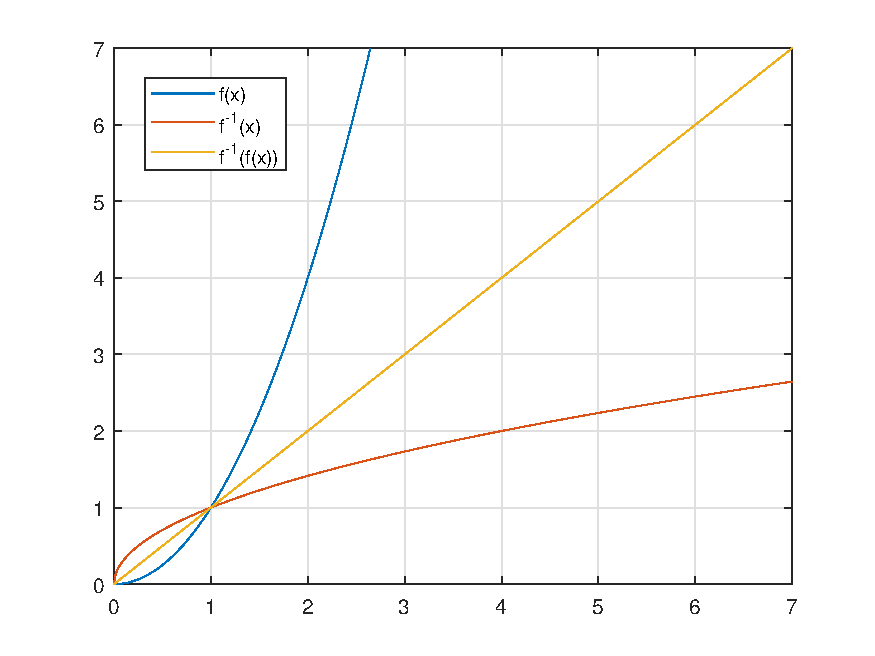
\includegraphics[width = 0.8\textwidth]{fig/Inversa-eps-converted-to.pdf}
}{O autor}{fig:fun_generica}{}{Função $f(x)$, sua inversa $f^{-1}(x)$ e a composição $f^{-1}(f(x))$ representadas de forma gráfica.}

Essa relação pode ser facilmente observada através da \autoref{fig:bijetividade}, sendo o primeiro conjunto o domínio da função $f$ e o segundo conjunto o contradomínio desta, enquanto para a função $f^{-1}$ essa relação se inverte.
\imagem{Função bijetiva e sua inversa}{
\resizebox{0.5\textwidth}{!}{
\label{fig:bijetividade}
\begin{tikzpicture}[->,thick]
 \node (a) at (0,0.5) {$A$};
 \node (b) at (0,0) {$B$};
 \node (c) at (0,-0.5) {$C$};
 \node[draw, ellipse, minimum height=2.5cm,minimum width=1.5cm, fit=(a) (b) (c)] {};
  
\node (d) at (2,0.5) {$X$};
\node (e) at (2,0) {$Y$};
\node (f) at (2,-0.5) {$Z$};
\node[draw, ellipse, minimum height=2.5cm,minimum width=1.5cm, fit=(d) (e) (f)] {};

\draw  (c) edge (f);
\draw  (b) edge (e);
\draw  (a) edge (d);
\node at (1,1.5) {$f$};

\node (a) at (0,-2.75) {$X$};
\node (b) at (0,-3.25) {$Y$};
\node (c) at (0,-3.75) {$Z$};
\node[draw, ellipse, minimum height=2.5cm,minimum width=1.5cm, fit=(a) (b) (c)] {};
  
\node (d) at (2,-2.75) {$A$};
\node (e) at (2,-3.25) {$B$};
\node (f) at (2,-3.75) {$C$};
\node[draw, ellipse, minimum height=2.5cm,minimum width=1.5cm, fit=(d) (e) (f)] {};

\draw  (c) edge (f);
\draw  (b) edge (e);
\draw  (a) edge (d);
\node at (1,-1.75) {$f^{-1}$};

\end{tikzpicture}
}
}{O autor}{fig:bijetividade}{}{Função bijetiva $f$ e sua inversa $f^{-1}$.}

A função do PA, portanto, desta perspectiva, não é bijetiva, pois apresenta uma região não-monotônica na qual para diferentes elementos no contradomínio existem dois ou mais elementos no domínio desta, o que pode ser visto na \autoref{fig:perfil_pa}. Nesta figura também é possível observar que a maior parte do modelo do PA é monotônico e crescente, ou seja, desconsiderando-se os efeitos de memória, essa parte da função é passível de possuir uma inversa.

\imagem{Perfil de um PA}{
\label{fig:perfil_pa}
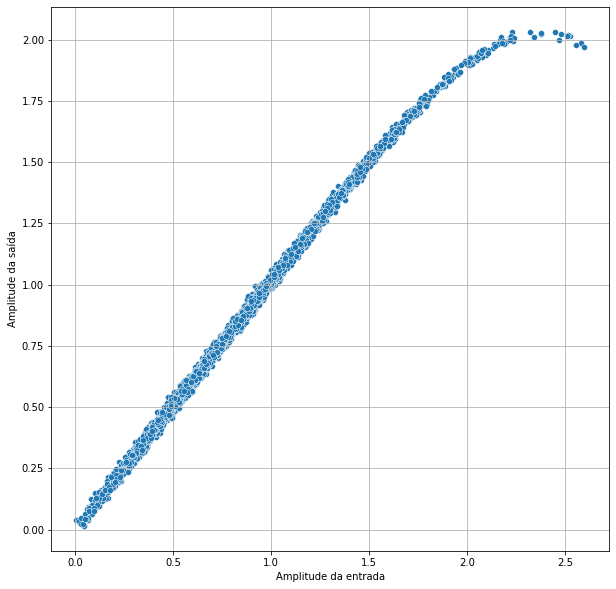
\includegraphics[width = 0.8\textwidth]{fig/modelo_pa.png}
}{O autor}{fig:perfil_pa}{}{Perfil de um PA, com os valores normalizados, mostrando sua região não-linear na região com entradas e saídas com maiores amplitudes.}

Apesar da função inversa do PA não ser única, a presença de elementos de memória que afetam o estado atual se torna uma condição de contorno para determinar o valor correto para a inversa em razão das entradas atuais e passadas. Na modelagem da inversa do PA, por meio da topologia presente neste trabalho, essa informação se torna implícita no modelo de caixa preta utilizado.

\section{Distorção digital} \label{sec:fundteo-distor}
O termo utilizado para o processo de linearização de PAs é distorção digital, tendo em vista os sinais a serem enviados são distorcidos pela inversa do PA ainda na etapa digital do processamento, antes de serem convertidos em sinais analógicos. Sendo um modo de conciliar a eficiência e a linearidade do PA, os distorcedores digitais podem ser separados em duas categorias básicas: Os pré-distorcedores digitais (DPDs) e os pós-distorcedores digitais (PoDs).

Um pré-distorcedor digital é um sistema pré-inverso, que distorce o sinal antes desse passar pela PA, conforme a \autoref{fig:dpd_cascata}. Enquanto o pós-distorcedor digital (PoD) é uma pós-inversa, que distorce o sinal após a passagem do mesmo pelo PA, como mostrado na \autoref{fig:pod_cascata}. Embora ambos sejam funções inversas do PA, o uso de PoD é inviável na prática devido a altas potências presentes na saída do PA.

\imagem{Cascata do DPD com o PA}{
\resizebox{0.8\textwidth}{!}{
\label{fig:dpd_cascata}
\begin{tikzpicture}[->,thick]
		\draw[-,blue]  plot[smooth, tension=.7] coordinates {(0.8,0.1) (1.3,0.6) (1.6,0.7)};
		\draw[-,red]  plot[smooth, tension=.7] coordinates {(-2.2,0.1) (-1.7,0.6) (-1.6,0.9)};
        \draw  (-2.5,1) rectangle node {DPD} (-1,0);
        \draw  (0.5,1) rectangle node {PA} (2,0);
        \draw (2,0.5) --  (3,0.5) node[above] {\tiny Saída} node[below] {\tiny medida};
        \draw (-1,0.5) -- node[above] {\tiny Incógnita} (0.5,0.5);
        \draw (-3.5,0.5) node[above] {\tiny Entrada} -- (-2.5,0.5);
        \node[circle, fill,minimum size=1.5mm,inner sep=0pt,outer sep=0pt] at (-3.5,0.5) {};
\end{tikzpicture}
}
}{O autor}{fig:dpd_cascata}{}{Cascata do DPD com o PA.}


\imagem{Cascata do PoD com o PA}{
\resizebox{0.8\textwidth}{!}{
\label{fig:pod_cascata}
\begin{tikzpicture}[->,thick]
        \draw[-,blue]  plot[smooth, tension=.7] coordinates {(-2.2,-1.4) (-1.7,-0.9) (-1.4,-0.8)};
		\draw[-,red]  plot[smooth, tension=.7] coordinates {(0.8,-1.4) (1.3,-0.9) (1.4,-0.6)};
        \draw  (-2.5,-0.5) rectangle node {PA} (-1,-1.5);
        \draw  (0.5,-0.5) rectangle node {PoD} (2,-1.5);
        \draw (2,-1) -- (3,-1) node[above] {\tiny Réplica linear} node[below] {\tiny da entrada};
        \draw (-3.5,-1) node[above] {\tiny Entrada} -- (-2.5,-1);
        \draw (-1,-1) -- node[above] {\tiny Saída} node[below] {\tiny medida} (0.5,-1);
        \node[circle, fill,minimum size=1.5mm,inner sep=0pt,outer sep=0pt] at (-3.5,-1) {};
\end{tikzpicture}
}
}{O autor}{fig:pod_cascata}{}{Cascata do DPD com o PA.}

Para os projetos do DPD e PoD, dois conjuntos de entradas e saídas medidas precisam estar disponíveis: um para o treinamento e outro para a validação. O projeto do PoD é uma modelagem computacional clássica na qual todas as informações do PoD são conhecidas. As informações para o PoD são obtidas pela troca de papeis da entrada e da saída do PA. Entretanto, por causa de sua saída desconhecida, projetar um DPD requer uma maior complexidade em relação ao PoD.

No que concerne ao treinamento do DPD, para contornar o treinamento direto mais pesado do DPD, uma arquitetura para um aprendizado indireto (ILA) é usualmente adotada. Na ILA, os parâmetros do modelo de PoD são primeiro identificados para um cenário mais clássico, no qual ambos os sinais de entrada e saída são conhecidos, e então os parâmetros são copiados para um modelo de DPD com a mesma topologia \cite{changsoo_eun_new_1997}.

No entanto, uma validação de DPD mais confiável exige o seu uso como um modelo pré-inverso. Por essa razão, na literatura é usualmente requerida uma nova medição do PA após o treinamento, como visto em \cite{8891388}. Neste método, uma sequência pré-distorcida é aplicada como a entrada do PA para a medição de sua saída. A saída do PA é então comparada com o sinal de entrada do DPD e o erro entre a entrada da cascata e o sinal de saída é calculado.

\section{Modelagem} \label{sec:fundteo-model}
O treinamento e a validação dos PAs e suas inversas fazem parte do campo da modelagem computacional, no qual estes sistemas são representados por modelos matemáticos que simulam seu comportamento. Neste trabalho uma abordagem caixa preta foi utilizada, que possui como característica usar um modelo cujos coeficientes não possuem uma relação física com o funcionamento do sistema e só busca reproduzir o comportamento \cite{8882211}.

Outra opção seriam modelos caixa branca, nos quais as funções presentes no modelo fazem referência direta ao comportamento do sistema ou aos seus componentes internos. Estes modelos possuem a vantagem no fato de seus coeficientes possuem significados físicos, no entanto o seu desenvolvimento pode ser mais demorado e só podem ser usados para representar sistemas físicos cujo comportamento é bem conhecido \cite{8882211}.

No caso das funções inversas, por não serem circuitos eletrônicos previamente existentes, os modelos caixa branca não são uma opção presente e o comportamento das mesmas deve ser reproduzido através de modelos caixa preta.

Em ambos os casos, a uma das principais funções de um modelo é prover um substituto às medições físicas, decorrente do fato das medições físicas onerarem em tempo, recursos e espaço. A utilização de modelos permite a realização de análises de forma mais prática.
Dentre as diversas técnicas de modelagem caixa preta, como as séries polinomiais, foi escolhido para este trabalho o uso de redes neurais artificiais do tipo perceptron de multicamada (MLP) em uma topologia específica para valores complexos.


%

% PARTE DOS REFERENCIAIS TEÓRICOS
% ----------------------------------------------------------
%\part{Referenciais teóricos}
%\chapter{Modelagem com redes neurais artificiais} \label{cha:model}

\section{Conceitos básicos} \label{sec:model-basic}

As redes neurais artificiais (ANN) são um tipo representativo dos modelos baseados na biologia, nos quais comportamentos e estruturas biológicas são reproduzidos através de funções e algoritmos, e, entre estes modelos, os algoritmos genéticos, de inteligência de enxame e as redes neurais artificiais se destacam pelo uso disseminado em diversas áreas da engenharia \cite{Darwish2018} \cite{Fan2020}.

A base das redes neurais artificiais é o perceptron, um modelo matemático do funcionamento dos neurônios presentes em nossos cérebros. Como passo inicial na analogia entre os perceptrons e os neurônios, os neurônios podem ser divididos, de modo muito simplificado, em três partes: os dendritos, o corpo e o axônio \cite{hall_tratado_2011}.

Os dendritos compõem os terminais de recepção do neurônio, no qual sinais provenientes de outros neurônios são recebidos e enviados para o corpo do neurônio. No corpo os sinais recebidos sofrem uma transformação não-linear e então são transmitidos para outros neurônios por meio do axônio.

De forma análoga, conforme a \autoref{fig:model-perceptron}, o perceptron é composto por uma região de recepção, da aplicação de uma função não-linear aos sinais de entradas e de uma etapa de transmissão para a camada seguinte de perceptrons. Através desta estrutura, o perceptron consegue separar qualquer região através de um plano n-dimensional \cite{haykin1999neural}.

\imagem{Modelo de perceptron}{
\resizebox{0.8\textwidth}{!}{
\begin{tikzpicture}[thick]
    \node[functions] (center) {$\tanh(.)$};
    \node[below of=center,font=\scriptsize,text width=4em] {\tiny Função de ativação};

    \node[right=2em of center] (right) {};
        \path[draw,->] (center) -- (right);
    
    \node[functions,left=2em of center] (left) {$\sum\limits_{i=1}^{N}(in_{i}w_{i})+b$};
        \path[draw,->] (left) -- (center);
    
    \node[weights,left=3em of left] (2) {$w_2$} -- (2) node[left of=2] (l2) {$in_2$};
        \path[draw,->] (l2) -- (2);
        \path[draw,->] (2) -- (left);
    \node[below of=2] (dots) {$\vdots$} -- (dots) node[left of=dots] (ldots) {$\vdots$};
    
    \node[weights,below of=dots] (n) {$w_N$} -- (n) node[left of=n] (ln) {$in_N$};
        \path[draw,->] (ln) -- (n);
        \path[draw,->] (n) -- (left);
    \node[weights,above of=2] (1) {$w_1$} -- (1) node[left of=1] (l1) {$in_1$};
        \path[draw,->] (l1) -- (1);
        \path[draw,->] (1) -- (left);
    
    \node[weights,above of=1] (0) {$b$} -- (0) node[left of=0] (l0) {$1$};
        \path[draw,->] (l0) -- (0);
        \path[draw,->] (0) -- (left);
    
    \node[below of=ln,font=\scriptsize] {\tiny Entradas};
    \node[below of=n,font=\scriptsize] {\tiny Pesos};
\end{tikzpicture}
}
\label{fig:model-perceptron}
}{O autor}{fig:model-perceptron}{}{Modelo de perceptron utilizando a função tangente hiperbólica como função de ativação.}

De forma mais detalhada, a \autoref{fig:model-perceptron} recebe um número $N$ de entradas e possui os pesos $w_i$ e o viés $b$ como coeficientes ajustáveis. As entradas são multiplicadas pelos pesos conforme os seus índices e então uma função não-linear, no caso deste trabalho a tangente hiperbólica, é aplicada ao resultado da soma das entradas ponderadas com o viés $b$. Esse processo também pode ser representado de forma matricial através da multiplicação de dois vetores, o que pode ser visto na equação \ref{eq:equacao_perceptron}, e então da aplicação da função não-linear.

\begin{align}
\begin{bmatrix}
1 \\ 
in_{1}\\ 
\vdots\\ 
in_{n}
\end{bmatrix}^{T}
\begin{bmatrix}
b\\ 
w_{1}\\ 
\vdots\\ 
w_{n}
\end{bmatrix}
=
\sum\limits_{i=1}^{n}
in_{i} \times w_{i} + b
\label{eq:equacao_perceptron}
\end{align}

Dentre as funções não-lineares usadas nas redes neurais artificiais as mais usadas são as funções sigmoides, ReLU e swish, em comum elas possuem características como serem monotônicas e uma região limitada de saída \cite{Szandaa2020}. A tangente hiperbólica faz parte das funções sigmoides e pode ser visualizada na \autoref{fig:tanh}, possuindo uma região de saída os valores entre -1 e 1 e sendo derivável em todos os seus pontos.

\imagem{Função tangente hiperbólica}{
\label{fig:tanh}
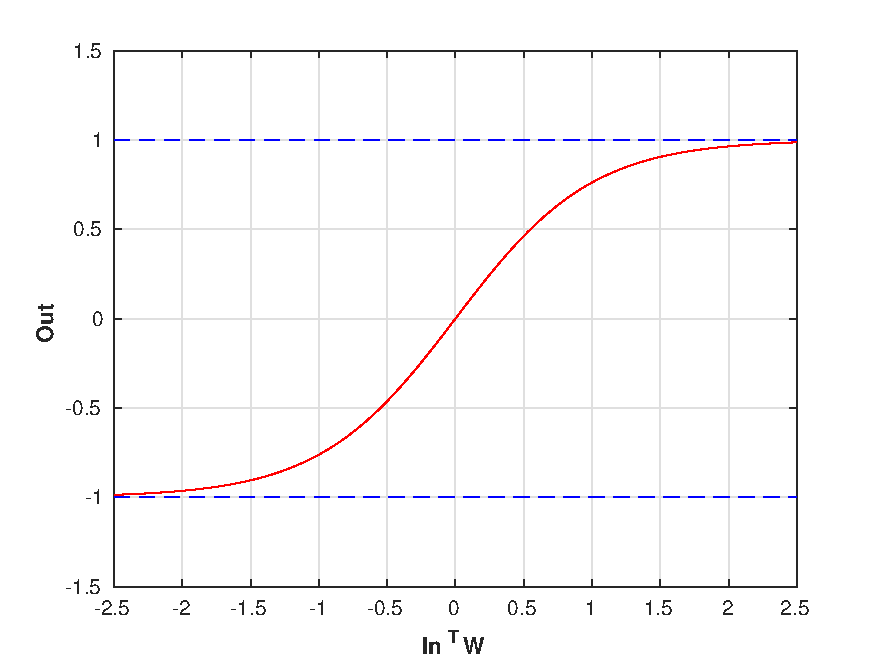
\includegraphics[width = 0.8\textwidth]{fig/sigmoide-eps-converted-to.pdf}
}{O autor}{fig:tanh}{}{Função tangente hiperbólica.}

Enquanto os perceptrons conseguem separar uma região através de um hiperplano, eles não possuem individualmente a capacidade de reproduzir funções mais complexas \cite{haykin1999neural}. Para isso é necessário usar os perceptrons reunidos em camadas, no que é conhecido como perceptron de multicamada (MLP), no qual a camada de entrada recebe os dados, passa esses para as camadas ocultas de perceptrons e no final estes dados são passados para a camada de saída também composta por perceptrons e que adequa os dados para as dimensões e para o intervalo correto. O MLP possui em sua versão mais simples uma única camada oculta e é conhecido como perceptron de três camadas (TLP), que pode ser visto na figura (), que possui a capacidade de representar qualquer função através de um número arbitrário de coeficientes \cite{Hornik1991}.
\ExplSyntaxOn
\NewDocumentCommand{\storedata}{mm}{\tl_set:Nn#1{#2}}
\DeclareExpandableDocumentCommand{\getdata}{O{1}m}{\tl_item:Nn#2{#1}}
\ExplSyntaxOff
\def\layersep{2cm}
\storedata\mydata{{$in_{1}$}{$in_{2}$}{$in_{3}$}{$in_{4}$}{$in_{5}$}}

\imagem{Perceptron de três camadas}{
\label{fig:tlp}
\resizebox{0.8\textwidth}{!}{
\begin{tikzpicture}[shorten >=1pt,->,draw=black, node distance=\layersep]
    \tikzstyle{every pin edge}=[<-,shorten <=1pt]
    \tikzstyle{neuron}=[circle,draw=black,minimum size=13pt,inner sep=5pt,font=\footnotesize]
    \tikzstyle{annot} = [text width=4em, text centered]

    % Draw the input layer nodes
    \foreach \name / \y in {1,...,5}
        \node[neuron, pin=left:{\small\getdata[\y]\mydata},fill=green] (I-\name) at (0,-0.8*\y) {};

    % Draw the hidden layer nodes
    \foreach \name / \y in {1,...,7}
        \path[yshift=0.15cm]
            node[neuron,fill=cyan] (H-\name) at (\layersep,-0.65*\y cm) {};

    % Draw the output layer node
    \node[neuron, right of=H-4,yshift=0.0cm,fill=red] (O) {};

    % Connect every node in the input layer with every node in the hidden layer.
    \foreach \source in {1,...,5}
        \foreach \dest in {1,...,7}
            \path (I-\source) edge 
            node[circle] {}(H-\dest);

    % Connect every node in the hidden layer with the output layer
    \foreach \source in {1,...,7}
        \path (H-\source) edge node[circle] {}(O);
        

     %Annotate the layers
    \node[annot,above of=H-1, node distance=0.70cm] (hl) {\small \textit{Oculta}};
    \node[annot,left of=hl] {\small \textit{Entrada}};
    \node[annot,right of=hl] {\small \textit{Saída}};
\node[coordinate,right of=O,node distance=1cm] (wabba){};
\draw [->] (O) -- node[above] {\small $Out_{1}$}(wabba);
\end{tikzpicture}
}
}{O autor}{fig:tlp}{}{Diagrama de blocos de um \textit{perceptron} de três camadas.}

Assim como o funcionamento do perceptron pode ser individualmente representado através de operações matriciais, conforme a equação \autoref{eq:equacao_perceptron}, as operações de uma camada de perceptrons pode ser representada por meio da multiplicação do vetor de entradas pela matriz composta pelos coeficientes da camada, como pode ser visto na \autoref{eq:camada_oculta}, aonde N é o número de entradas e H o número de perceptrons na camada, e então pela aplicação da função de ativação para cada um dos membros do vetor de saída.

\begin{align}
\begin{bmatrix}
1 \\ 
in_{1}\\ 
\vdots\\ 
in_{N}
\end{bmatrix}^{T}
\begin{bmatrix}
b_{0}   & b_{1}   & \hdots & b_{H} \\ 
w_{1,0} & w_{1,1} & \hdots & w_{1,H} \\ 
\vdots  & \vdots  & \ddots & \vdots \\ 
w_{N,0} & w_{N,1} & \hdots & w_{N,H}
\end{bmatrix}
=
\begin{bmatrix}
\sum\limits_{i=1}^{n} in_{i} \times w_{i,0} + b_{0}\\ 
\sum\limits_{i=1}^{n} in_{i} \times w_{i,1} + b_{1}\\ 
\vdots\\ 
\sum\limits_{i=1}^{n} in_{i} \times w_{i,H} + b_{H}
\end{bmatrix}^{T}
\label{eq:camada_oculta}
\end{align}

\section{Treinamento e validação} \label{sec:model-trei}
Enquanto o teorema universal de aproximação informa que as o TLP pode aproximar qualquer função continua com os um conjunto arbitrário de coeficientes, esse número de coeficientes pode ser extremamente alto e a busca destes coeficientes não é coberta por esse teorema \cite{Goodfellow-et-al-2016}. Para se obter um conjunto de coeficientes que consiga generalizar uma função ainda é necessário que o processo de treinamento convirja para esse resultado através das consecutivas iterações, o mais conhecido entre os processos de treinamento para os coeficientes de uma rede neural artificial com múltiplas camadas é o processo conhecido como \textit{backpropagation}, que foi um dos primeiros algoritmos a conseguir ajustar de forma eficiente os coeficientes das camadas ocultas \cite{Goodfellow-et-al-2016} \cite{6302929}. Após o surgimento do \textit{backpropagation} outros algoritmos para o treinamento dos coeficientes foram encontrados \cite{Khidirova2020} \cite{Escalante2006}, o algoritmo utilizado nesse trabalho para o treinamento dos coeficientes foi o Levenberg–Marquardt \cite{Marquardt1963}.

Independente do algoritmo de treinamento utilizado, o processo de treinamento supervisionado de uma rede neural artificial requer um conjunto de amostras de entrada e de saída, sendo que no caso do treinamento de sistemas com memória as amostras devem estar organizadas temporalmente. O processo de treinamento realiza um ajuste iterativo dos coeficientes, normalmente utilizando as informações do gradiente das respostas, em busca de valores que minimizem uma função de perda que implique na aproximação do modelo ao sistema utilizado. De modo geral, os valores iniciais dos coeficientes podem ser escolhidos de maneira aleatória.

Como o modelo é treinado com um número finito de dados, é necessária a validação do mesmo com um segundo conjunto de entradas e saídas. A validação é essencial para garantir que não ocorram efeitos como o overfitting, no qual o modelo se ajusta perfeitamente a um conjunto específico de dados, mas não é capaz de reproduzir de maneira consistente o comportamento fora deste escopo \cite{haykin1999neural}. O conjunto de dados da validação é aplicado de forma a extrair os resultados da função de perda, a mesma função utilizada no treinamento.

Outras métricas podem ser usadas adicionalmente para se avaliar o comportamento do modelo durante e após o treinamento, neste trabalho a principal métrica utilizada foi o erro quadrático médio normalizado (NMSE), expresso através da \autoref{eq:nmse}.

\begin{align}
NMSE = 10\log_{10}
\left(
\frac
{\sum\limits_{i=1}^{N}
\abs{O_{i}-\widehat{O}_{i}}^{2}}
{\sum\limits_{i=1}^{N}
\abs{O_{i}}^2}
\right)
\label{eq:nmse}
\end{align}

\section{Topologia utilizada} \label{sec:model-topo}
Uma das principais características dos sinais dos amplificadores de potência é a sua representação por meio da utilização de números complexos, em razão disso o modelo utilizado deve possuir uma arquitetura capaz de representar os valores em suas componentes de amplitude e fase ou a partir da representação retangular. Em ambos os casos dois valores reais são necessários para representar cada amostra de entrada ou de saída do sinal.

Nesse trabalho a arquitetura utilizada, proposta em \cite{chipansky_freire_modfied_2015}, utiliza dois TLP para a extração da parte real e imaginária conforme a \autoref{fig:model-topo}. O modelo recebe o valor absoluto $a_x$ e a fase $\theta_x$ do sinal de entrada, assim como os valores passados numa profundidade de memória $M$. Os $M+1$ valores absolutos são passados diretamente como entrada para as duas redes neurais, enquanto as $M+1$ fases são usadas para determinar $M$ mudanças de fases conforme a equação \autoref{eq:diff_fase}, na qual $n$ é o número da amostra e $m$ assume os valores entre $0$ e $M$. As diferenças de fases são passadas como entradas para as funções senos e cossenos, para então estes valores tomarem seu lugar como entradas para os dois TLP.
%\criarsimbolo{$\angle$}{Fase de um número complexo}\label{item:fase}

\begin{align}
\Delta\theta_x(n,m) = \theta_x(n-m+1)-\theta_x(n-m)
\label{eq:diff_fase}
\end{align}

\imagem{Topologia utilizada}{
\resizebox{0.8\textwidth}{!}{
\begin{tikzpicture}[shorten <=0.1pt,shorten >=0.1pt,>=stealth,thick,->]

\draw  (-2,3.9) rectangle node {TLP} (-0.85,5.95);
\draw  (-2,7.1) rectangle node {TLP} (-0.85,9.15);

\draw  [thick,->,>=stealth] (-7.75,9) -- (-2,9);

\node [circle,minimum size=1.5mm,inner sep=0pt,outer sep=0pt,fill=black] at (-2.5,9) {};
\node [circle,minimum size=1.5mm,inner sep=0pt,outer sep=0pt,fill=black] at (-3,8.3) {};
\node[circle,minimum size=1.5mm,inner sep=0pt,outer sep=0pt,fill=black] at (-3.25,7.95) {};
\node[circle,minimum size=1.5mm,inner sep=0pt,outer sep=0pt,fill=black] at (-3.5,7.6) {};
\node[circle,minimum size=1.5mm,inner sep=0pt,outer sep=0pt,fill=black] at (-3.75,7.25) {};
\node  [circle,minimum size=1.5mm,inner sep=0pt,outer sep=0pt,fill=black] at (-2.75,8.65) {};
\node[circle,minimum size=1.5mm,inner sep=0pt,outer sep=0pt,fill=black] at (-6,9) {};
\node [circle,minimum size=1.5mm,inner sep=0pt,outer sep=0pt,fill=black] at (-5.5,7.35) {};
\node[circle,minimum size=1.5mm,inner sep=0pt,outer sep=0pt,fill=black] at (-5,5.5) {};

\draw (-2.5,9) -- (-2.5,5.8) -- (-2,5.8);

\draw (-6,7.75) -- (-6,7.6) -- (-5,7.6) -- (-5,8.65) -- (-2,8.65);

\draw (-7.75,7.35) -- (-4.75,7.35) -- (-4.75,8.3) -- (-2,8.3);

\draw (-2.75,8.65) -- (-2.75,5.45) -- (-2,5.45);
\draw (-3,8.3) -- (-3,5.1) -- (-2,5.1);
\draw (-5.5,6.25) -- (-5.5,6.1) -- (-4.5,6.1) -- (-4.5,7.95) node (v3) {} -- (-2,7.95);

\draw (-3.25,7.95) -- (-3.25,4.75) -- (-2,4.75);
\draw (-3.5,7.6) -- (-3.5,4.4) -- (-2,4.4);
\draw (-3.75,7.25) -- (-3.75,4.05) -- (-2,4.05);

\draw (-7.75,5.5) -- (-4.25,5.5) -- (-4.25,7.6) -- (-2,7.6);
\draw (-5,4.4) -- (-5,4.25) -- (-4,4.25) -- (-4,7.25) -- (-2,7.25);
\draw (-0.85,7.75) -- (0.15,7.75) node[above]{$\Re[\tilde{s}(n)]$} -- (0.15,6.55);
\draw (-0.85,4.55) --  (0.15,4.55) node[below] {$\Im[\tilde{s}(n)]$}-- (0.15,4.85);

\draw  (0.15,6.3) ellipse (0.25 and 0.25);
\draw (0.4,6.3) -- (0.9,6.3);
\draw (1.15,7) -- (1.15,6.55);
\draw  (1.15,6.3) ellipse (0.25 and 0.25);
\draw (1.4,6.3) -- node[above] {\~y(n)} (2.15,6.3);
\draw  (-0.35,5.6) rectangle node{j(.)} (0.65,4.85);
\draw (0.15,5.6) -- (0.15,6.05);
\draw  (0.65,7.75) rectangle node {$e^{j(.)}$} (1.65,7);
\draw (1.15,8.15) -- (1.15,7.75);
\draw  (-5.5,5.15) rectangle node {$Z^{-1}$} (-4.5,4.65);
\draw  (-6,7) rectangle node {$Z^{-1}$} (-5,6.5);
\draw  (-6.5,8.5) rectangle node {$Z^{-1}$} (-5.5,8);

\draw (-5.5,7.35) -- (-5.5,7);
\draw (-6,9) -- (-6,8.5);
\draw (-5,5.5) -- (-5,5.15);

\draw[dotted,-] (-6,8) -- (-6,7.75);
\draw[dotted,-] (-5.5,6.5) -- (-5.5,6.25);
\draw[dotted,-] (-5,4.65) -- (-5,4.4);

\node at (-7.75,8.75) {$a_{x}(n)$};
\node at (-7.75,7) {$cos(\Delta\theta_x(n,1))$};
\node at (-7.75,5.15) {$sin(\Delta\theta_x(n,1))$};

\node at (-7,7.75) {$a_{x}(n-M)$};
\node at (-7,6.25) {$cos(\Delta\theta_x(n,M))$};
\node at (-6.5,4.25) {$sin(\Delta\theta_x(n,M))$};

\node at (0.15,6.3) {\textbf{+}};
\node at (1.15,6.3) {$\times$};

\node [circle,minimum size=1.5mm,inner sep=0pt,outer sep=0pt,fill=black] at (-7.75,9) {};
\node [circle,minimum size=1.5mm,inner sep=0pt,outer sep=0pt,fill=black] at (-7.75,7.35) {};
\node [circle,minimum size=1.5mm,inner sep=0pt,outer sep=0pt,fill=black] at (-7.75,5.5) {};
\node [circle,minimum size=1.5mm,inner sep=0pt,outer sep=0pt,fill=black,above] at (1.15,8.15) {};
\node at (1.15,8.5) {$\theta_{x}(n)$};
\end{tikzpicture}}
\label{fig:model-topo}
}{O autor}{fig:model-topo}{}{Diagrama de blocos de um modelo de DPD baseado no TLP.}


% PARTE DOS RESULTADOS
% ----------------------------------------------------------
%\part{Resultados}
%\chapter{Estudo de caso - Parte I} \label{cha:estudoi}
\section{PA analisado} \label{sec:estudoi-pa}
Neste estudo de caso foram utilizados os dados extraídos de um modelo Advanced Memory Polynomial (AMP) com um sinal LTE com 153,6 MHz. O AMP foi treinado para representar o esquemático de um PA multímodo proposto para a tecnologia CMOS 130 nm, operando no sexto modo e possuindo uma frequência central de 2,4 GHz largura de banda de 20 MHz, com a frequência de amostragem de 153,6 MHz \cite{dos2017fully} \cite{schuartz2019reduced}. Para os dados de treinamento foram utilizadas 3000 amostras, enquanto 2000 amostras foram utilizadas nas etapas de validação.

\section{Ferramentas} \label{sec:estudoi-ferr}
Diversas ferramentas existem para o desenvolvimento de modelos computacionais, neste estudo de caso foi escolhida como ferramenta principal a linguagem de programação Python. Python é uma linguagem de programação multiparadigma e com alto nível de abstração, que permite a utilização de bibliotecas construídas em linguagens de programação mais eficientes na utilização dos recursos computacionais como C/C++, Fortran e Rust \cite{Ramalho2022-zg}.

Para a construção dos TLPs, foi utilizada a biblioteca TensorFlow, com o auxílio da biblioteca Keras para a construção dos modelos através de sua API funcional. Desenvolvida pelo Google utilizando-se C++, o TensorFlow é uma biblioteca para a criação e o treinamento de projetos de aprendizagem de máquina, com foco em redes neurais artificiais \cite{tensorflow2015-whitepaper}.

Para a representação dos valores, foi utilizada a biblioteca Numpy, construída utilizando-se C. Trata-se de uma biblioteca voltada para a computação cientifica através do uso de matrizes de valores numéricos \cite{harris2020array}.

Para a resolução dos problemas de otimização de forma a encontrar as soluções do problema inverso, a biblioteca utilizada foi a Scipy, construída utilizando-se principalmente Python, Fortran e C \cite{2020SciPy-NMeth}.

A biblioteca Polars, construída em Rust, foi utilizada para a representação dos dados em formado tabular. Para a visualização destes dados, as bibliotecas Matplotlib e Seaborn foram utilizadas \cite{Hunter:2007} \cite{Waskom2021}.

\section{Metodologia} \label{sec:estudoi-meto}
O primeiro passo para obtenção dos resultados é a construção do modelo do PA utilizando-se dois TLPs na topologia apresentada, o modelo foi construído em Python e os TLPs foram construídos utilizando-se as bibliotecas TensorFlow e Keras. Como parâmetros para a construção do modelo, foram especificadas a profundidade de memória M, a quantidade de perceptrons presentes na camada oculta HL e a função de ativação.

Para o treinamento do modelo, o método de otimização utilizado foi o Levenberg-Marquardt e como função de perda o erro quadrático médio (MSE). O treinamento foi efetuado através da função padrão presente na biblioteca TensorFlow. Como métrica para comparar os resultados do treinamento e da validação do modelo foi escolhido o NMSE.

Uma função representando o problema inverso foi criada de tal forma que, se o seu resultado foi zero, o processo de resolução do problema inverso seja exitoso. Essa função é responsável por receber o valor esperado para a saída do modelo e o valor proposto pelo método de resolução como entrada atual do modelo. A partir do valor proposto, ao ser passado ao modelo junto com as entradas passadas conhecidas, é encontrada a saída do modelo. A função retorna a diferença entre a saída obtida do modelo e a saída esperada multiplicada por um fator gama. Esse fator gama é igual a 1 caso a entrada proposta possua amplitude menor que 3 e é igual a amplitude da entrada proposta caso contrário.

Dois conjuntos de 9 entradas propostas foram criados, sendo a diferença entre eles a amplitude, o primeiro conjunto possuindo 0,5 como amplitude e o segundo 2,5. Enquanto as 9 fases escolhidas foram distribuídas de uniformemente ao redor do círculo unitário, iniciando-se em 0. Valores na \autoref{tab:valores}.
\tabela{valores iniciais utilizados}
{
\begin{tabular}{l|l|l}
\hline
    & \multicolumn{2}{c}{\textbf{Amplitude}} \\ \hline
    \textbf{Fase (rad)} & \textbf{0.5} & \textbf{2.5} \\ \hline
    \textit{0}& 0,5$\angle$0 & 2,5$\angle$0 \\ \hline
    \textit{2$\pi$/9} & 0,5$\angle$2$\pi$/9  & 2,5$\angle$2$\pi$/9  \\ \hline
    \textit{4$\pi$/9} & 0,5$\angle$4$\pi$/9  & 2,5$\angle$4$\pi$/9  \\ \hline
    \textit{6$\pi$/9} & 0,5$\angle$6$\pi$/9  & 2,5$\angle$6$\pi$/9  \\ \hline
    \textit{8$\pi$/9} & 0,5$\angle$8$\pi$/9  & 2,5$\angle$8$\pi$/9  \\ \hline
    \textit{10$\pi$/9}& 0,5$\angle$10$\pi$/9 & 2,5$\angle$10$\pi$/9 \\ \hline
    \textit{12$\pi$/9}& 0,5$\angle$12$\pi$/9 & 2,5$\angle$12$\pi$/9 \\ \hline
    \textit{14$\pi$/9}& 0,5$\angle$14$\pi$/9 & 2,5$\angle$14$\pi$/9 \\ \hline
    \textit{16$\pi$/9}& 0,5$\angle$16$\pi$/9 & 2,5$\angle$16$\pi$/9 \\ \hline
\end{tabular}
\label{tab:valores}
}
{O autor}{tab:valores}{}{Representação complexa dos valores iniciais utilizados em formato de amplitude e fase.}

A função \textit{optimize.root}, da biblioteca SciPy, foi utilizada para encontrar as raízes da função que representa o problema inverso. O método de otimização utilizado foi o HYBRD \cite{powell1970hybrid}.

Com os resultados de todas as entradas propostas obtidas para todas as amostras analisadas, duas informações são extraídas: O NMSE entre a saída esperada e a saída obtida e o NMSE entre a entrada esperada e a entrada obtida pela resolução do problema inverso. E é a partir destes resultados que as análises presentes neste relatório serão feitas, outras informações adicionais também serão utilizadas de forma complementar.

\section{Modelagem e validação do modelo do PA} \label{sec:estudoi-model}
Para o modelo de PA utilizado nesse estudo de caso, foi definida uma profundidade de memória M igual à 3 e um número de perceptrons na camada oculta HL igual à 7, totalizando-se 85 parâmetros para a parte real e mais 85 parâmetros para a parte imaginária do modelo.

\imagemH{Resultado do treinamento do modelo de PA}{
\label{fig:extracao_pa}
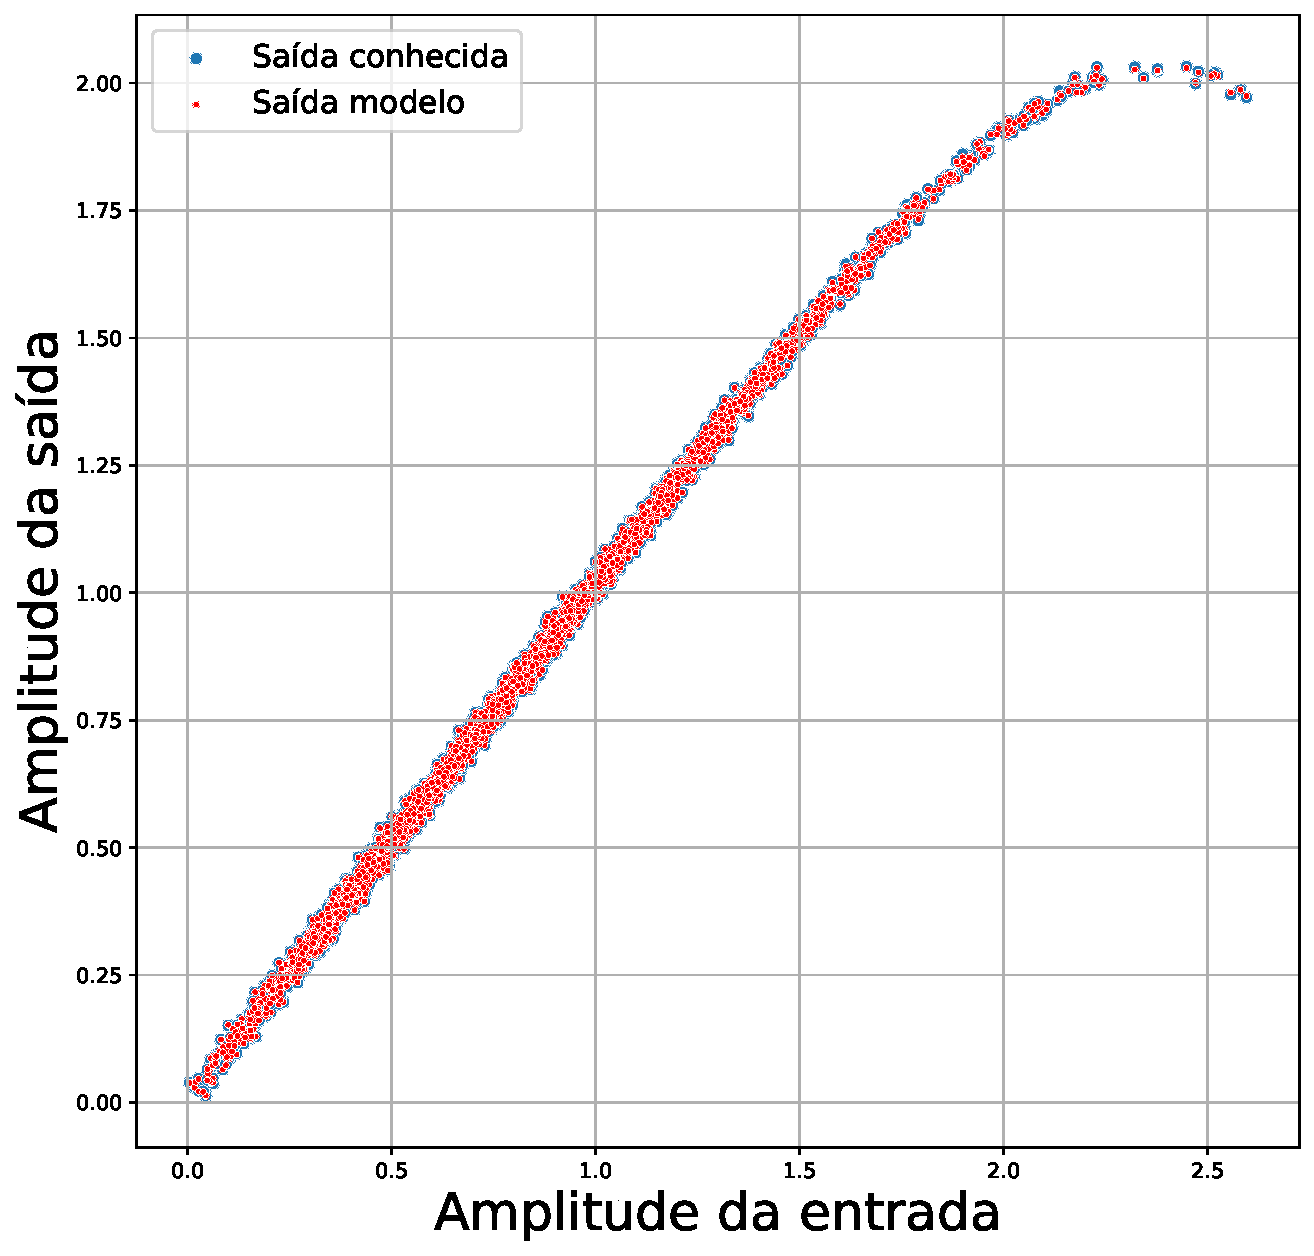
\includegraphics[width = 0.8\textwidth]{fig/extracao_pa.pdf}
}{O autor}{fig:extracao_pa}{}{Comparação gráfica entre as saídas conhecidas do PA e as saídas do modelo para os dados de treinamento.}

A função de ativação foi a tangente hiperbólica, o total de entradas foi igual a 10, na camada de saída foi utilizada uma função de ativação linear, para a busca dos coeficientes foi utilizada a métrica MSE e o processo de busca usou o algoritmo Levenberg-Marquardt. O treinamento das partes real e imaginária foi realizado separadamente.

O modelo foi capaz de ter um NMSE de -60.9 dB para os dados de treinamento e de -42.9 dB para os dados de validação. A \autoref{fig:extracao_pa} apresenta os valores da amplitude da saída em relação à entrada para os dados medidos e para os gerados pelo modelo para o conjunto de treinamento, enquanto a \autoref{fig:validacao_pa} mostra as mesmas informações para o conjunto de validação.

\imagem{Resultado da validação do modelo de PA}{
\label{fig:validacao_pa}
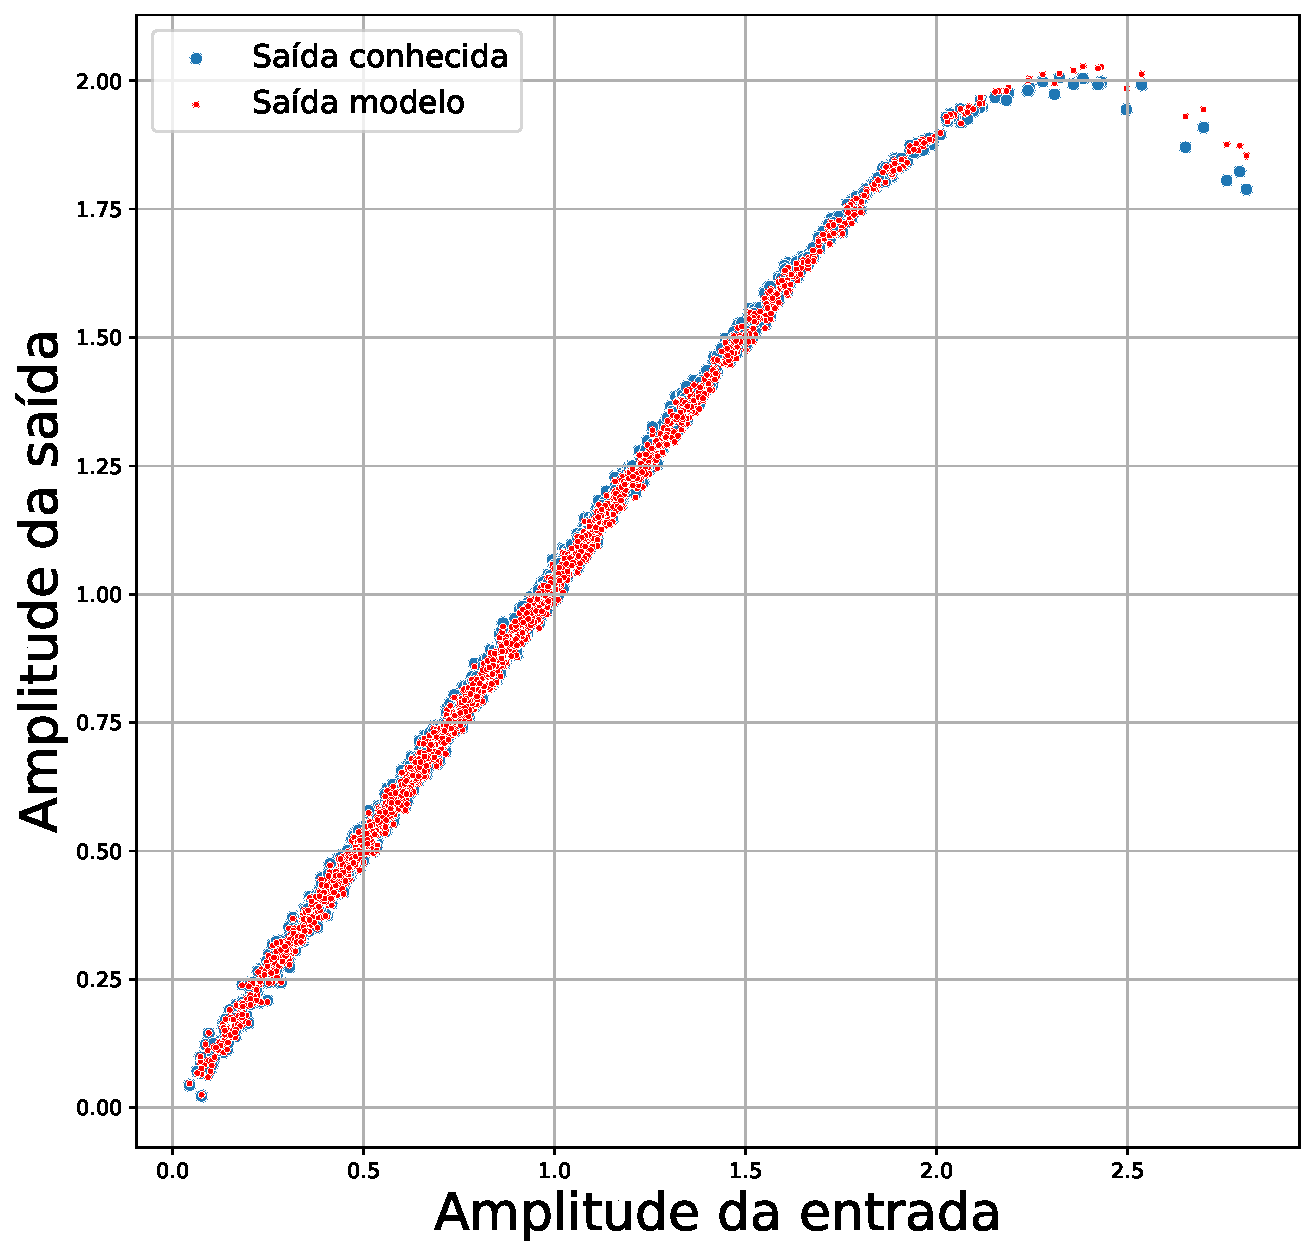
\includegraphics[width = 0.8\textwidth]{fig/validacao_pa.pdf}
}{O autor}{fig:validacao_pa}{}{Comparação gráfica entre as saídas conhecidas do PA e as saídas do modelo para os dados de validação.}

\section{Uso do PI na análise do comportamento} \label{sec:estudoi-pi}

\subsection{Efeitos da continuidade da ANN} \label{subsec:estudoi-pi-conti}
As redes neurais possuem a capacidade de generalizar o comportamento da função e estender esse comportamento para regiões não mapeadas. Isso causa uma complicação a mais, pois, mesmo para entradas de menor amplitude, uma região descrente e não mapeada pode ser formada, como visto na \autoref{fig:continuidade_pa}. Uma forma de mitigar este problema é penalizar a otimização na região não mapeada, multiplicando o erro encontrado por um coeficiente proporcional a amplitude de entrada proposto. O método de causar uma descontinuidade na região se mostrou ineficiente em testes preliminares e, portanto, não foi utilizado.

\imagem{Continuidade do modelo}{
\label{fig:continuidade_pa}
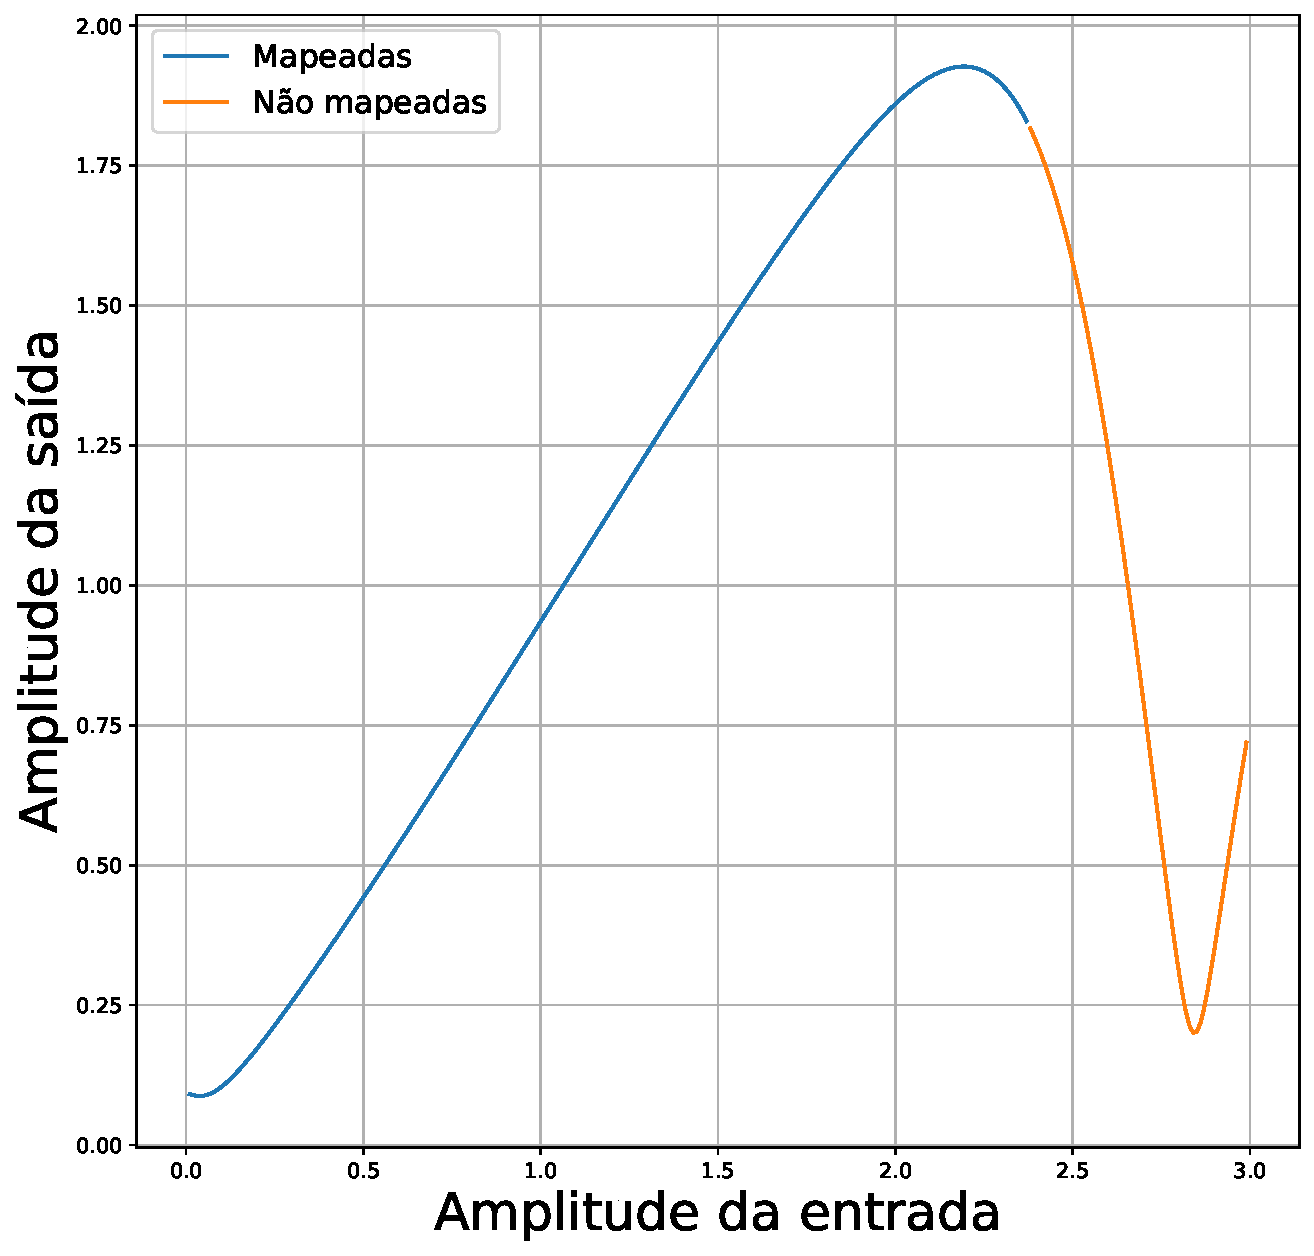
\includegraphics[width = 0.8\textwidth]{fig/continuidade_pa.pdf}
}{O autor}{fig:continuidade_pa}{}{Continuidade do modelo do PA com a memória fixa e variando-se a entrada entre 0 e 3, separando-se a região mapeada no treinamento e a região não mapeada no treinamento.}

\subsection{Efeito da amplitude dos valores iniciais no PI} \label{subsec:estudoi-pi-efeito}
Os 18 diferentes valores presentes na \autoref{tab:valores} foram definidos como valores iniciais para o processo de solução do problema inverso. Estes foram separados, juntamente aos resultados, em dois conjuntos: o primeiro conjunto com amplitude de 0,5 e segundo conjunto com amplitude de 2,5.

Nas \autoref{fig:erro_05} e \autoref{fig:erro_25} pode-se observar o comportamento destes dois principais conjuntos, no qual vemos a formação de três regiões. A região superior representa os valores que não convergiram, enquanto a inferior é dividida entre os que convergiram para os valor esperado e as que encontraram um valor de entrada não esperado. No gráfico está representado o erro entre os valores de saída e de entrada do modelo por meio do NMSE em dB.

\imagemH{Erros do PI para o valor inicial de 0,5}{
\label{fig:erro_05}
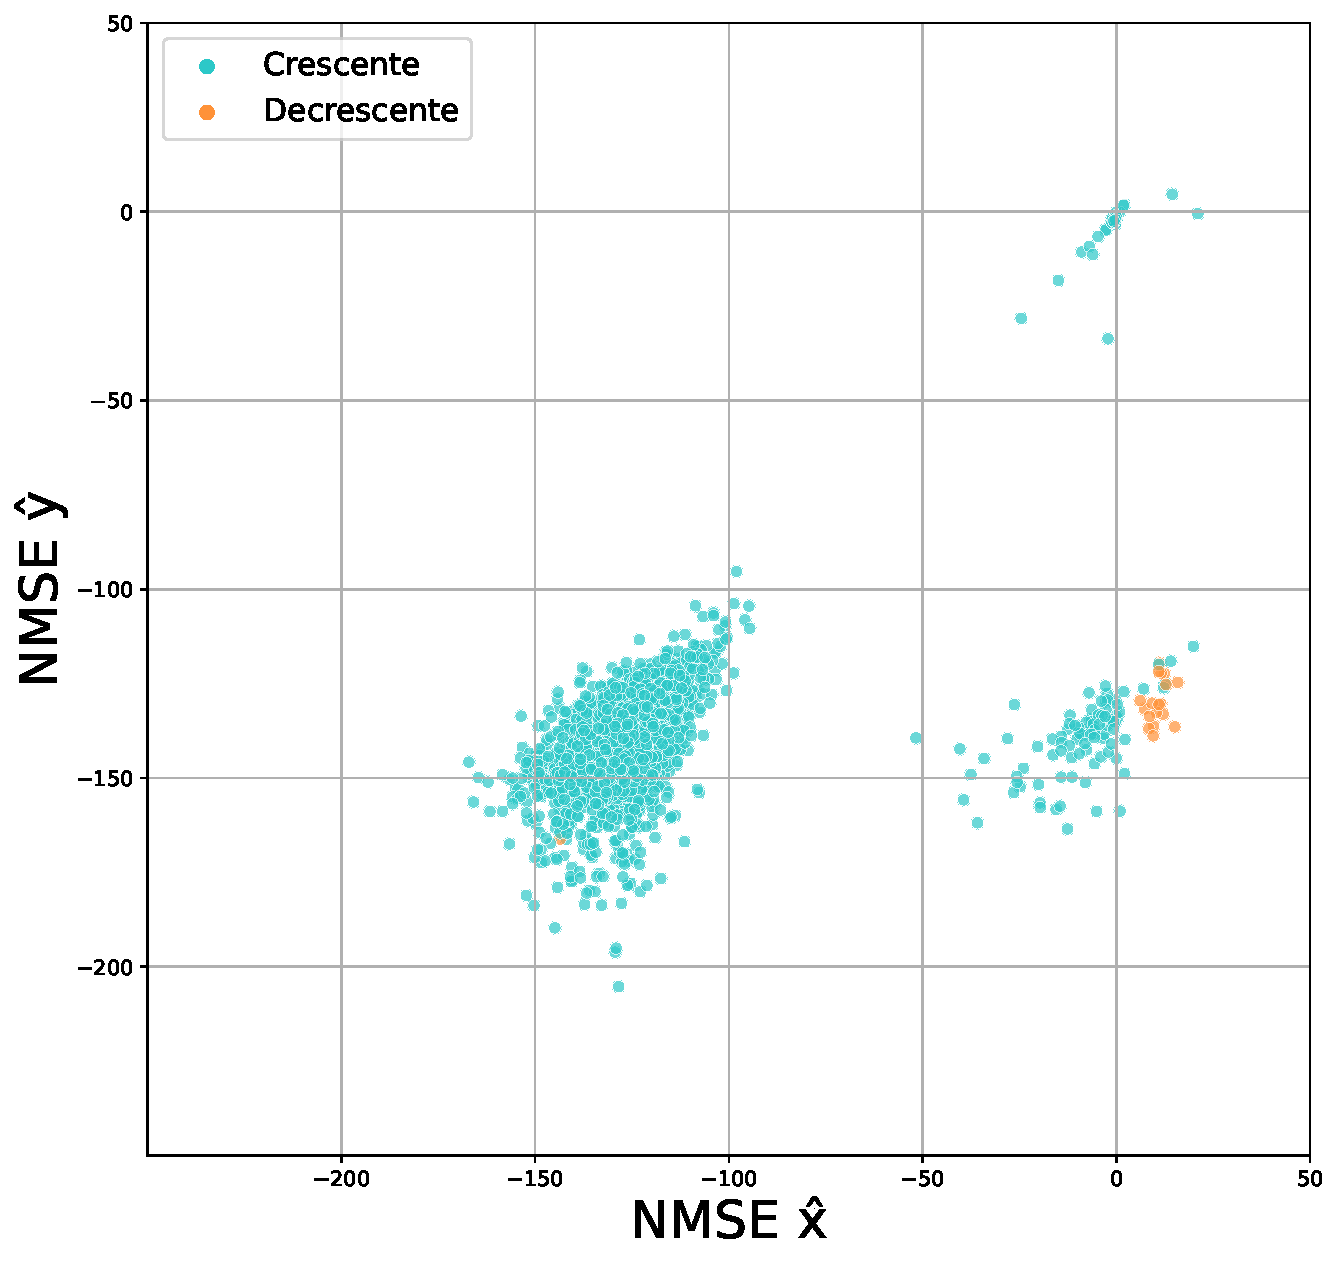
\includegraphics[width = 0.8\textwidth]{fig/erros_05.pdf}
}{O autor}{fig:erro_05}{}{Gráfico dos erros em dB da entrada e da saída das soluções do problema inverso, com os resultados divididos nos três grupos analisados, para uma amplitude de 0,5.}

\imagemH{Erros do PI para o valor inicial de 2,5}{
\label{fig:erro_25}
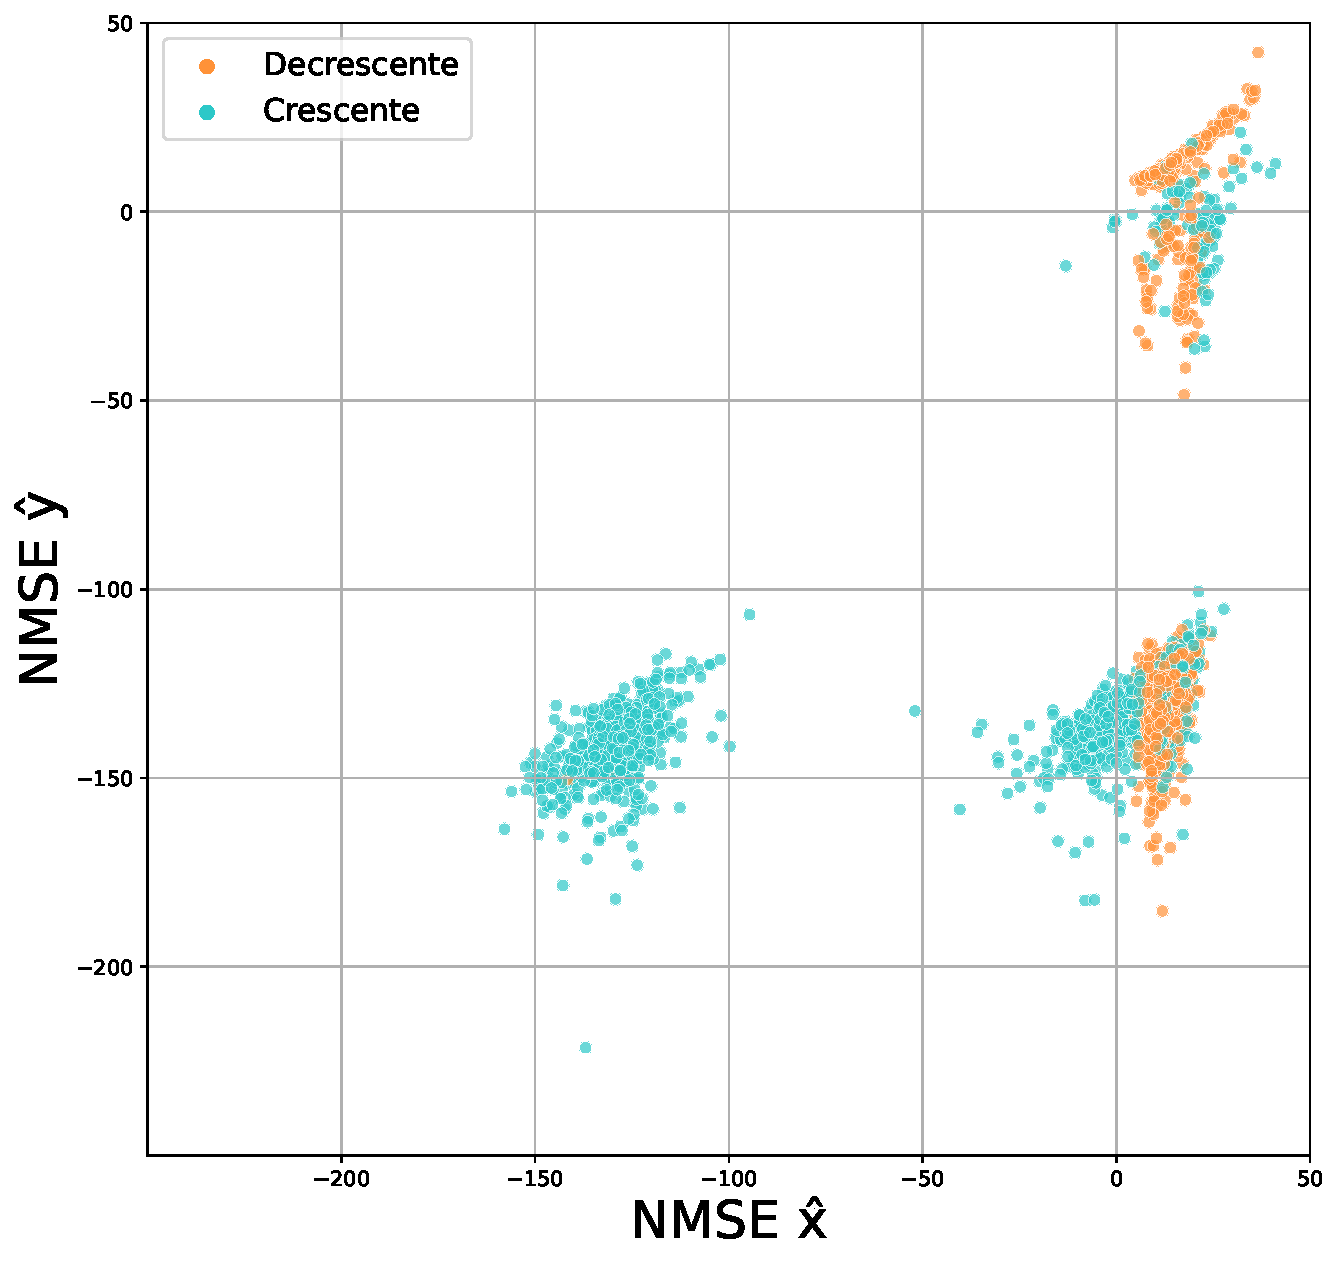
\includegraphics[width = 0.8\textwidth]{fig/erros_25.pdf}
}{O autor}{fig:erro_25}{}{Gráfico dos erros em dB da entrada e da saída das soluções do problema inverso, com os resultados divididos nos três grupos analisados, para uma amplitude de 2,5.}

A distribuição por amplitudes e fases pode ser vista na \autoref{tab:valores_resultados05} para a amplitude de 0,5 e na \autoref{tab:valores_resultados25} para a amplitude de 2,5.

\tabela{Resultados para a amplitude 0,5}{
\begin{tabular}{l|r|r|r}
    \hline
    \textbf{Valor inicial} & \textbf{Não convergiu} & \textbf{Falso} & \textbf{Correto} \\ \hline
    0,5$\angle$0 & 2,14\% & 3,14\% & 94,72\% \\ \hline
    0,5$\angle$2$\pi$/9 & 1,74\% & 3,51\% & 94,76\% \\ \hline
    0,5$\angle$4$\pi$/9 & 1,30\% & 3,71\% & 94,99\% \\ \hline
    0,5$\angle$6$\pi$/9 & 1,47\% & 3,04\% & 95,49\% \\ \hline
    0,5$\angle$8$\pi$/9 & 1,27\% & 3,67\% & 95,06\% \\ \hline
    0,5$\angle$10$\pi$/9 & 1,34\% & 3,27\% & 95,39\% \\ \hline
    0,5$\angle$12$\pi$/9 & 1,47\% & 4,18\% & 94,36\% \\ \hline
    0,5$\angle$14$\pi$/9 & 1,17\% & 3,97\% & 94,86\% \\ \hline
    0,5$\angle$16$\pi$/9 & 1,27\% & 4,04\% & 94,69\% \\ \hline
    \textbf{Média} & 1,46\% & 3,61\% & 94,92\% \\ \hline
    \end{tabular}
\label{tab:valores_resultados05}
}{O autor}{tab:valores_resultados05}{}{Resultados para a amplitude 0,5}

\tabela{Resultados para a amplitude 2,5}{
\begin{tabular}{r|l|l|l}
    \hline
        \textbf{Valor inicial} & \textbf{Não convergiu} & \textbf{Falso} & \textbf{Correto} \\ \hline
        2,5$\angle$0 & 16,70\% & 65,93\% & 17,37\% \\ \hline
        2,5$\angle$2$\pi$/9 & 15,36\% & 67,57\% & 17,07\% \\ \hline
        2,5$\angle$4$\pi$/9 & 15,76\% & 67,70\% & 16,53\% \\ \hline
        2,5$\angle$6$\pi$/9 & 17,33\% & 65,36\% & 17,30\% \\ \hline
        2,5$\angle$8$\pi$/9 & 16,83\% & 64,20\% & 18,97\% \\ \hline
        2,5$\angle$10$\pi$/9 & 17,74\% & 63,93\% & 18,34\% \\ \hline
        2,5$\angle$12$\pi$/9 & 16,13\% & 64,60\% & 19,27\% \\ \hline
        2,5$\angle$14$\pi$/9 & 14,96\% & 66,30\% & 18,74\% \\ \hline
        2,5$\angle$16$\pi$/9 & 15,90\% & 64,36\% & 19,74\% \\ \hline
        Média & 16,30\% & 65,55\% & 18,15\% \\ \hline
    \end{tabular}
\label{tab:valores_resultados25}
}{O autor}{tab:valores_resultados25}{}{}

\subsection{Efeito do valor inicial em uma única amostra} \label{subsec:estudoi-pi-entradas}
Após se explorar o comportamento de todas as amostras para dezoito entradas diferentes, foi realizada uma análise para uma única amostra com amplitude de entrada igual a 2,58 e amplitude de saída igual a 1,99. Para essa amostra, um total de 3600 entradas iniciais foram utilizadas, variando-se de forma constante o ângulo entre 0 e 6,18 radianos e a amplitude entre 0 e 2,95.

Na \autoref{fig:calor_todos} vemos a amplitude de entrada encontrada para as diferentes resoluções do problema inverso, em razão da amplitude e do ângulo do valor inicial.
\imagemH{Amplitudes das soluções do PI}{
\label{fig:calor_todos}
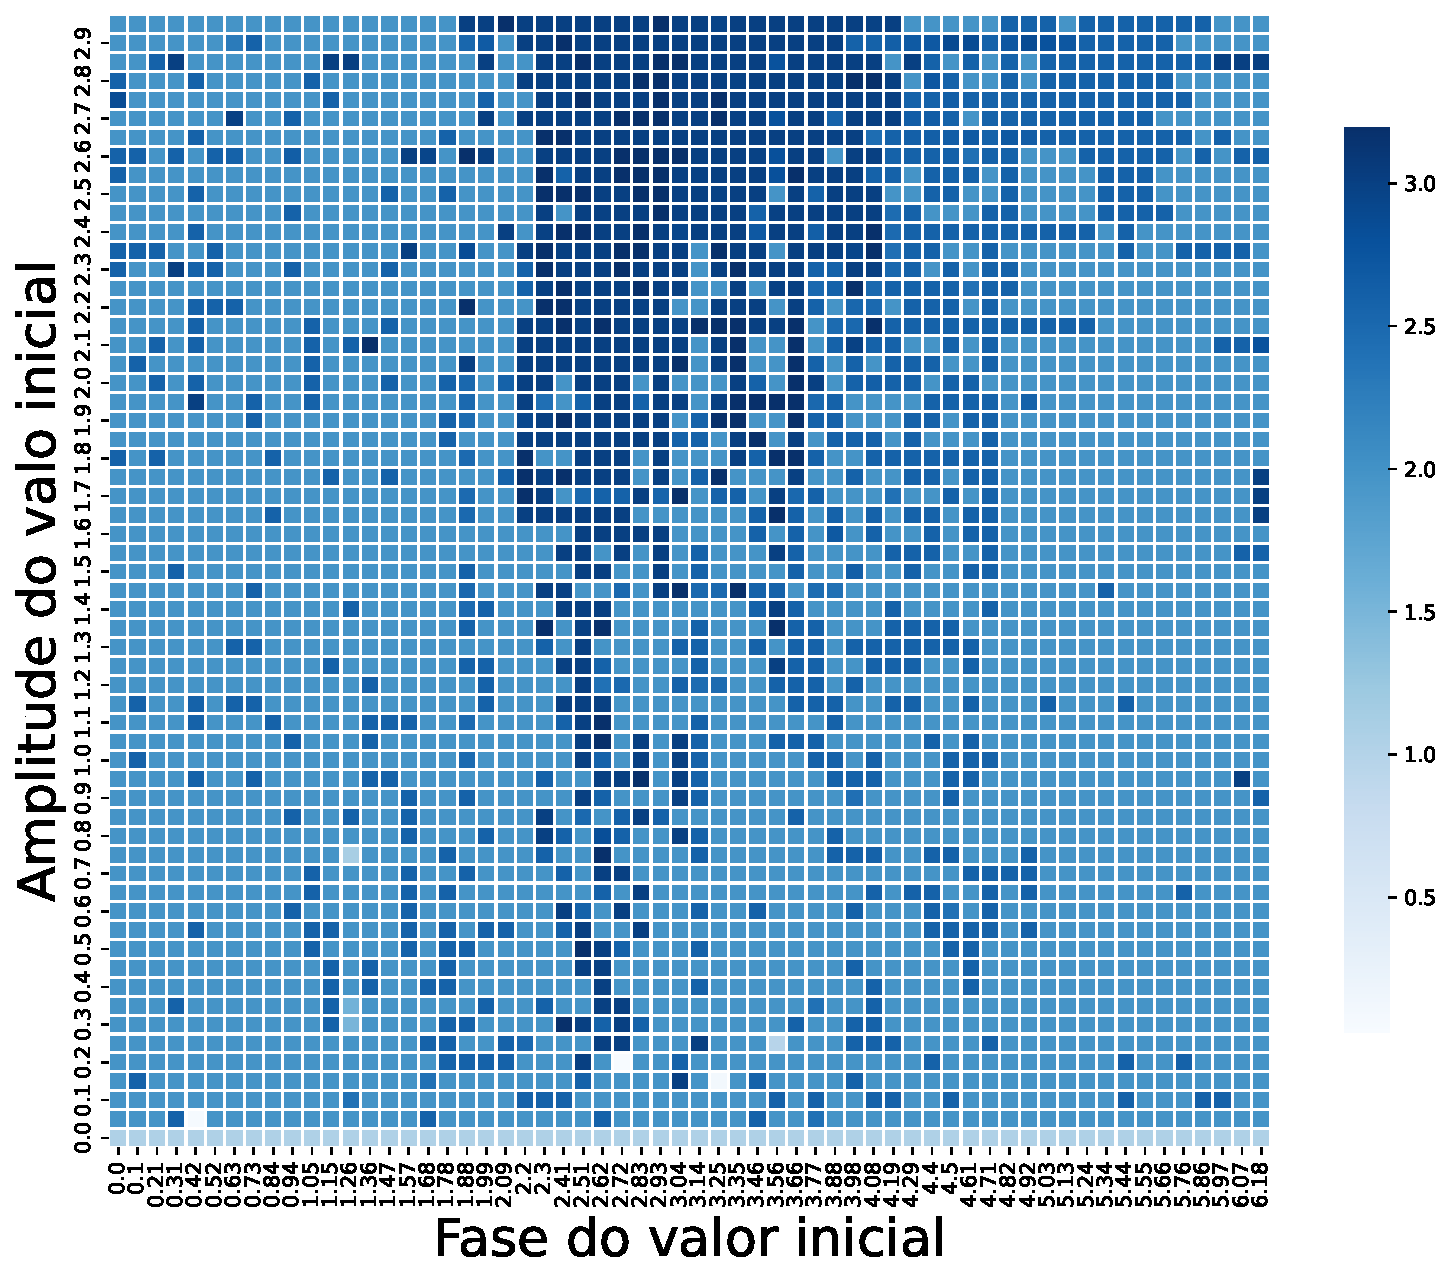
\includegraphics[width = 0.8\textwidth]{fig/calor_todos.pdf}
}{O autor}{fig:calor_todos}{}{Mapa de calor das amplitudes encontradas como soluções do PI para a entrada do modelo após a resolução do PI para diferentes valores iniciais.}

No entanto, é necessário se excluir os pontos em que não ocorreu uma convergência. Para isso analisamos o erro entre a saída do modelo e a saída ao ser aplicado o resultado do problema inverso, mostrado na \autoref{fig:calor_erro}.

\imagemH{Erros das soluções do PI}{
\label{fig:calor_erro}
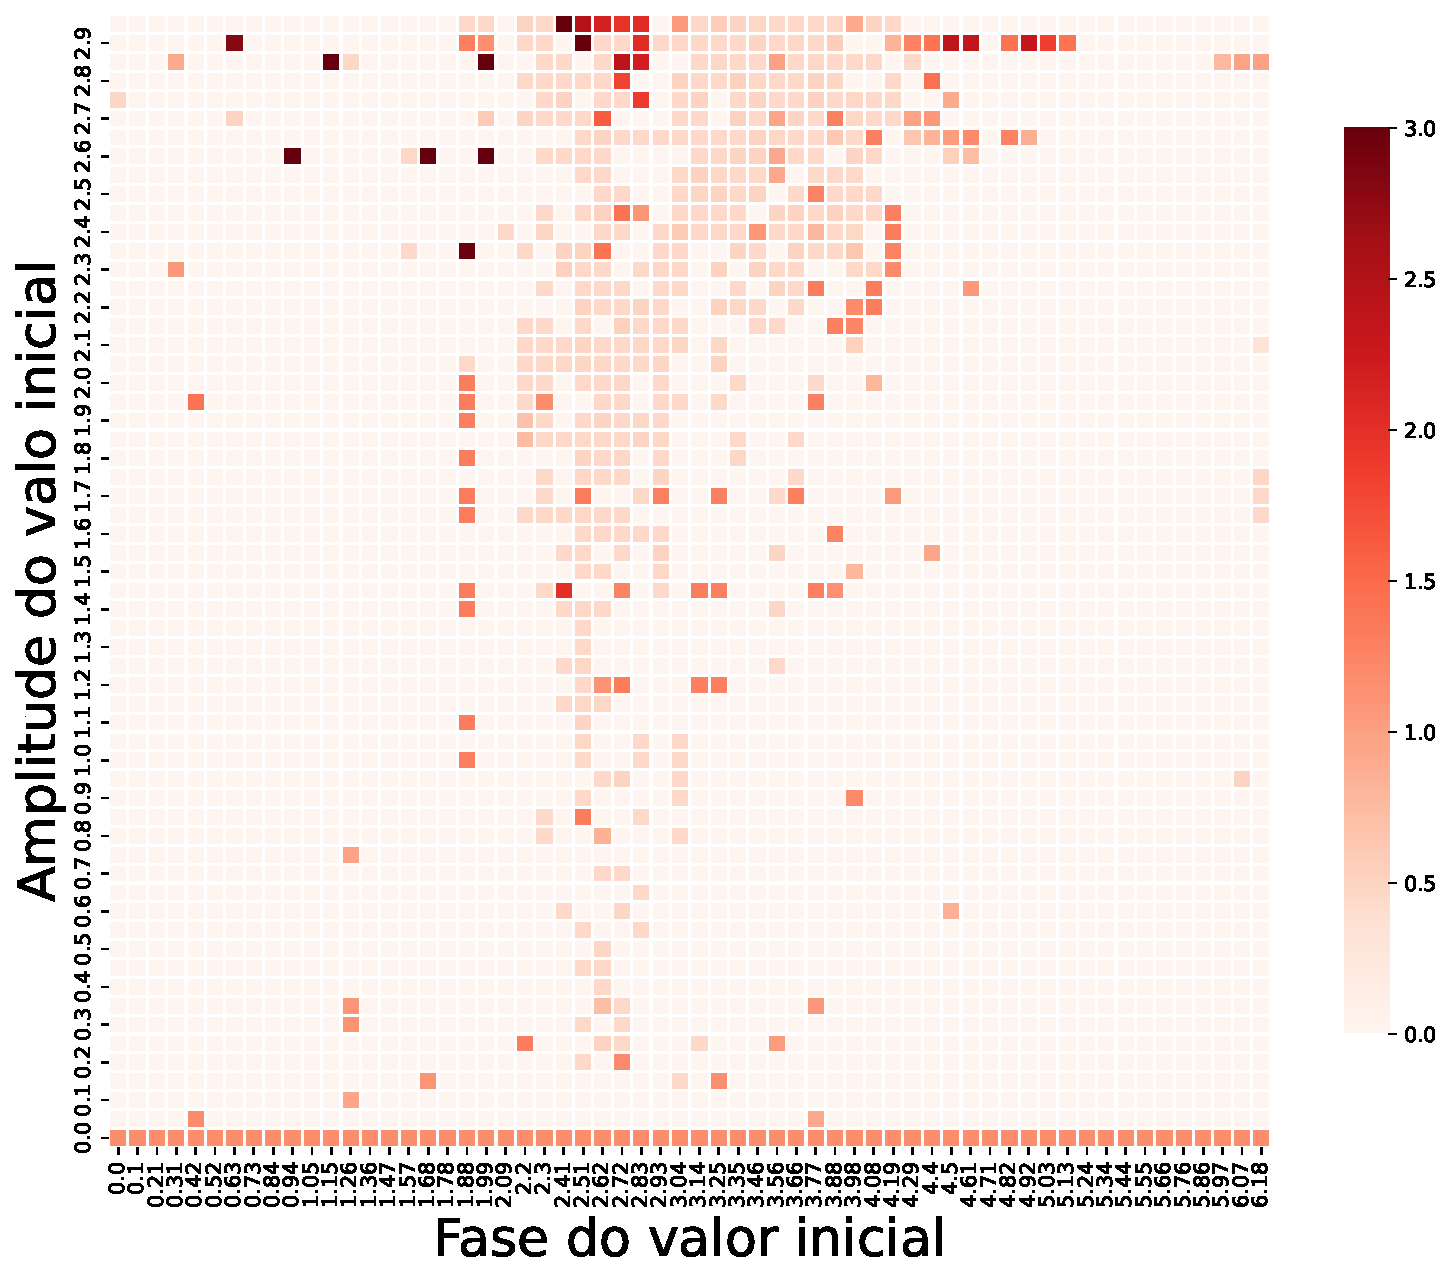
\includegraphics[width = 0.8\textwidth]{fig/calor_erro.pdf}
}{O autor}{fig:calor_erro}{}{Mapa de calor dos erros entre as saídas do modelo obtidas pela aplicação das soluções do PI e a saída do modelo obtida pela aplicação da entrada verdadeira.}

Após o processo de exclusão destas amostras, que produzem um formato similar a um triangulo, obtemos como resultado a \autoref{fig:calor_converge}, na qual podemos ver com clareza três resultados encontrados para a resolução do problema inverso, com o resultado correto sendo o prevalente para a maior parte dos pontos.

\imagemH{Amplitude das soluções convergentes do PI}{
\label{fig:calor_converge}
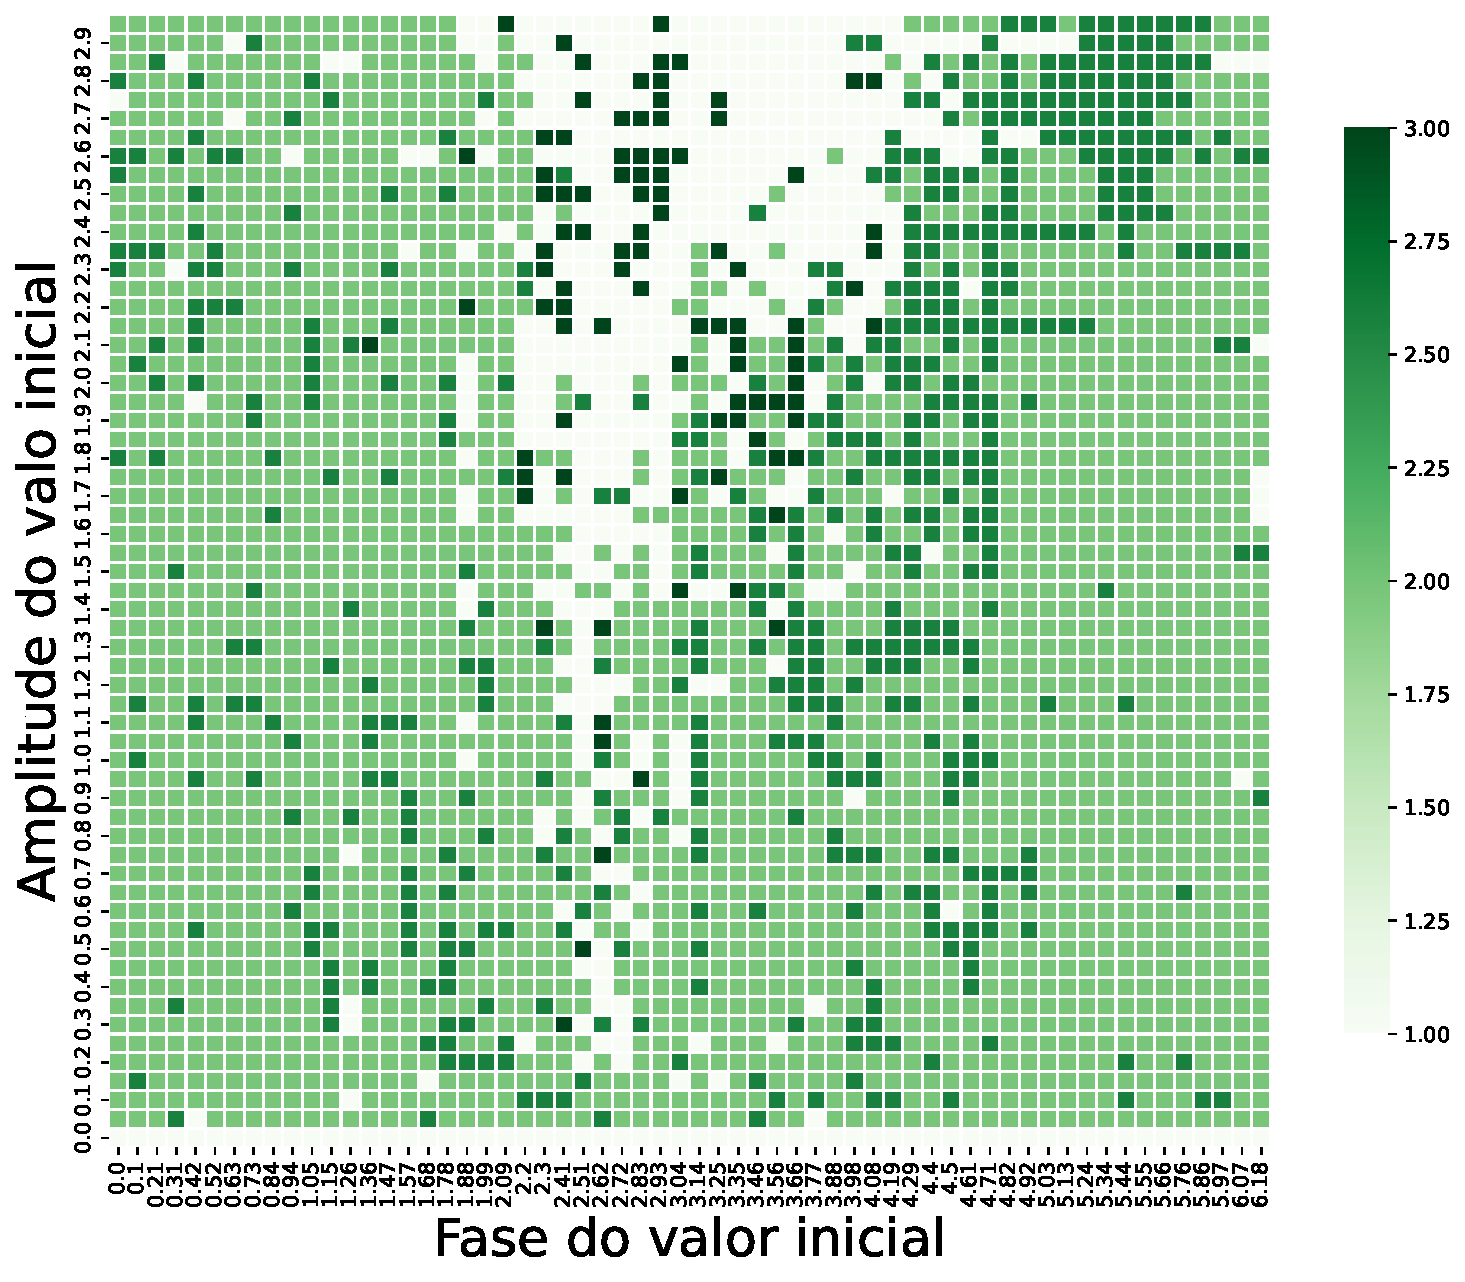
\includegraphics[width = 0.8\textwidth]{fig/calor_converge.pdf}
}{O autor}{fig:calor_converge}{}{Mapa de calor das amplitudes encontradas como soluções convergentes do PI para a entrada do modelo após a resolução do PI para diferentes valores iniciais.}

\section{Treinamento da inversa} \label{sec:estudoi-inv}
Os resultados práticos no treinamento da inversa do PA através da mesma topologia, utilizando um valor de profundidade de memória M igual à 3 e uma quantidade de perceptrons na camada oculta HL igual à 7, deixam clara a maior dificuldade que o modelo inverso possui para generalizar os resultados na região não-linear e que mesmo o resultado do treinamento apresenta um desemprenho inferior ao do modelo direto. Isso pode ser observado graficamente nas \autoref{fig:extracao_inversa} e \autoref{fig:validacao_inversa}, respectivamente, os dados de treinamento, com um NMSE de -51,33 dB, e de validação, com um NMSE de -26,48 dB.

\imagem{Resultado do treinamento da inversa do PA}{
\label{fig:extracao_inversa}
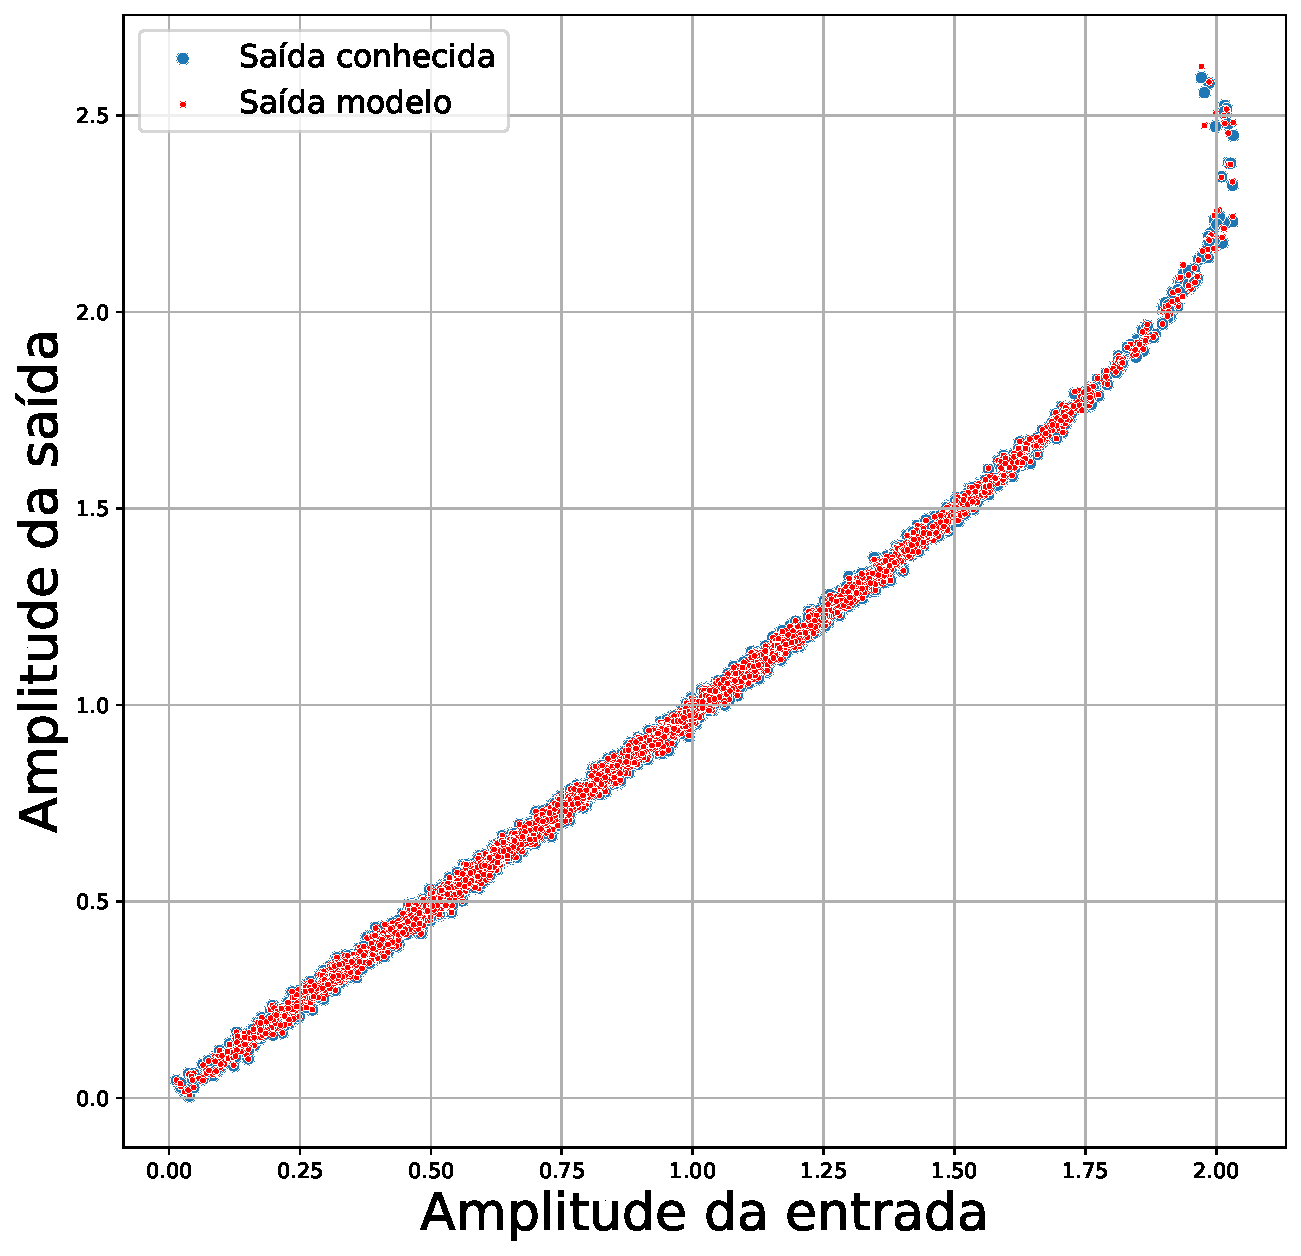
\includegraphics[width = 0.8\textwidth]{fig/extracao_inversa.pdf}
}{O autor}{fig:extracao_inversa}{}{Comparação gráfica entre as saídas conhecidas e as saídas do modelo da inversa do PA para os dados de extração.}

\imagem{Resultado da validação da inversa do PA}{
\label{fig:validacao_inversa}
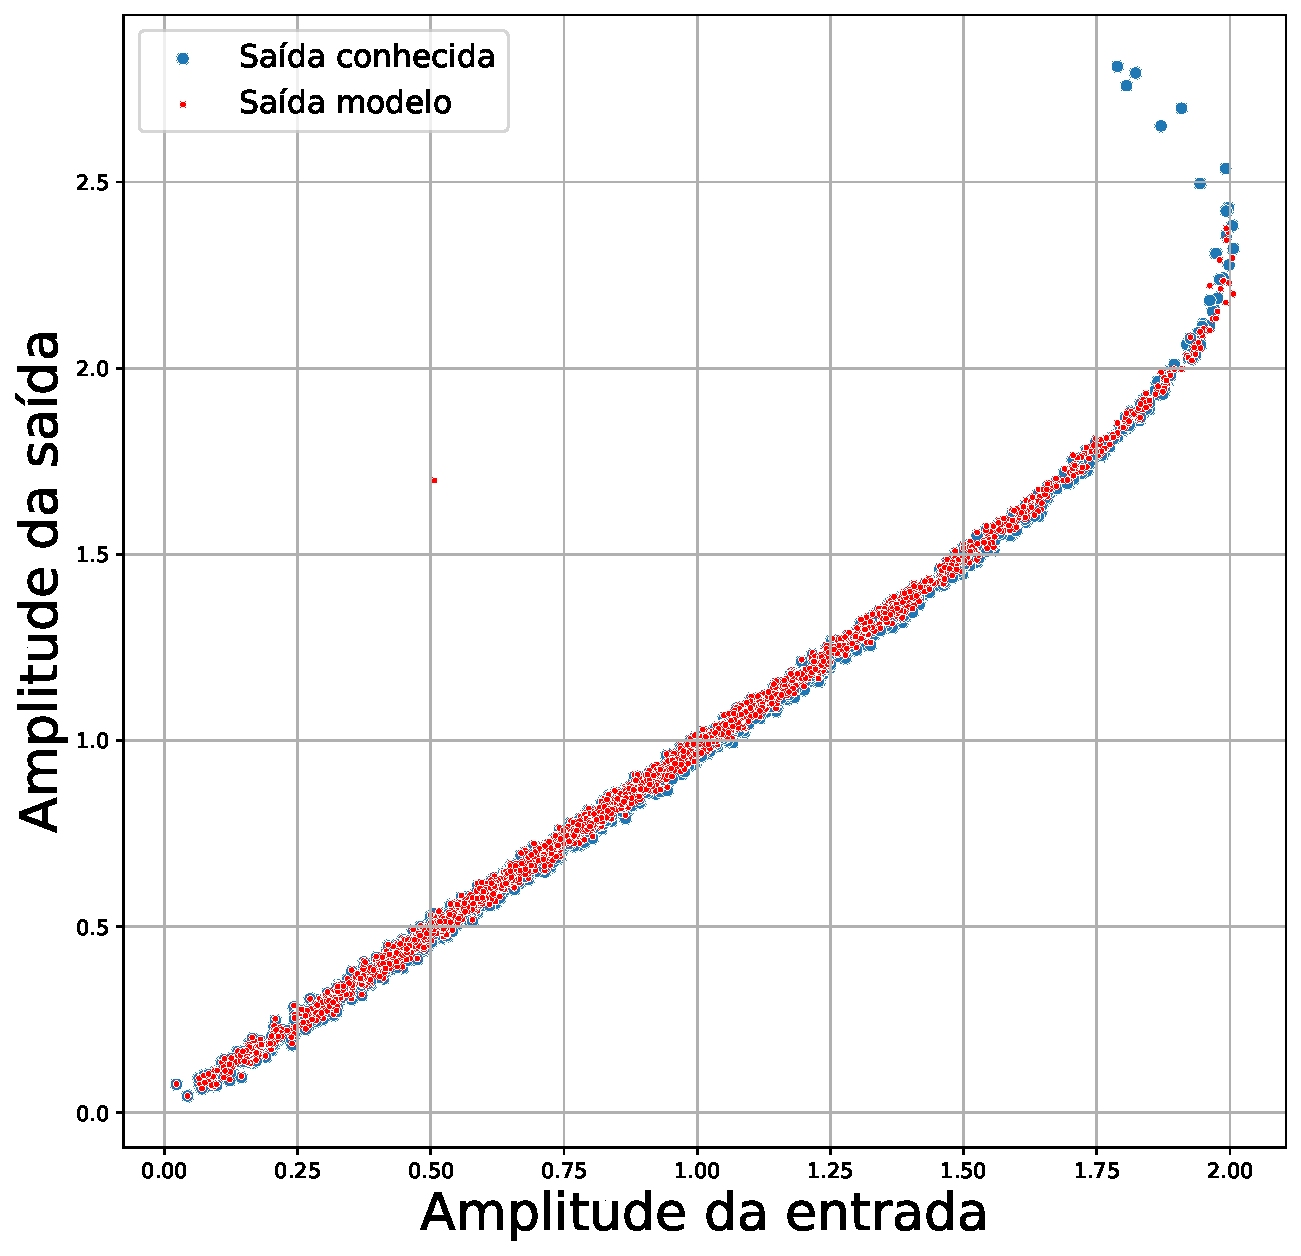
\includegraphics[width = 0.8\textwidth]{fig/validacao_inversa.pdf}
}{O autor}{fig:validacao_inversa}{}{Comparação gráfica entre as saídas conhecidas e as saídas do modelo da inversa do PA para os dados de validação.}


% Finaliza a parte no bookmark do PDF
% para que se inicie o bookmark na raiz
% e adiciona espaço de parte no Sumário
% ----------------------------------------------------------
%\phantompart

% ---
% Conclusão (outro exemplo de capítulo sem numeração e presente no sumário)
% ---
%\chapter*[Conclusão]{Conclusão}
%\addcontentsline{toc}{chapter}{Conclusão}
% ---
%\chapter{Estudo de caso - Parte II} \label{cha:estudoii}

A técnica de validação do DPD proposta neste trabalho pode ser aplicada para qualquer modelo de DPD. Nesta seção, como uma prova de conceito, {tal técnica é aplicada para a validação de DPDs para quatro PAs, sendo todos os quatro DPDs simulados por redes neurais de valores reais, porém cada um deles é treinado para um PA específico, possuindo um número diferente de entradas e de \textit{perceptrons} na camada oculta, o que altera drasticamente o número de coeficientes de cada um deles, conforme descreve a Seção V.A}. Os detalhes do problema inverso, que é utilizado nesse trabalho, são discutidos na Seção V.B. Os resultados são reportados na Seção V.C.

\section{PAs analisados} \label{sec:estudoii-pas}
Neste estudo de caso foram utilizados os dados...

\section{Ferramentas} \label{sec:estudoii-fer}
Matlab bla bla bla

\section{Validação do DPD por meio do PI} \label{sec:estudoii-dpd}
O método estabelecido na literatura para a validação da pré-inversa requer uma medição adicional do PA após o treinamento do DPD. O segundo estudo de caso deste trabalho tem o objetivo de oferecer uma alternativa que emprega somente as medições do PA coletadas antes do treinamento do DPD.

O método proposto precisa da geração de um sinal de saída do pré-distorcedor que seja igual às entradas previamente medidas no PA. Uma vez que, na estratégia proposta todas as medidas do PA são feitas antes do treinamento do DPD, o sinal de entrada do PA nunca será uma sequência pré-distorcida, sendo sempre um sinal não distorcido. Na estratégia proposta, busca-se obter uma entrada do DPD que idealmente seja uma réplica da saída medida no PA que, por sua vez, é um sinal distorcido. Como mostrado na \autoref{fig:pi-validacao}, o DPD e suas saídas são conhecidos, mas as entradas do DPD necessárias para gerar o sinal de saída do pré-distorcedor que é igual às entradas do PA previamente medidas são desconhecidas. Achar estas entradas descreve um problema inverso, representado pelo bloco $DPD^{-1}$ na \autoref{fig:pi-validacao}, que precisa de uma solução numérica para cada instante de tempo.

Para finalizar a validação, o erro entre as entradas estimadas, por meio da solução do problema inverso, do DPD e as saídas previamente medidas do PA é computado. Isso é equivalente a medir o erro entre a entrada da cascata e o sinal de saída, como mostrado na \autoref{fig:pi-validacao}. Visto que a saída da cascata deve apresentar uma relação linear com a entrada da mesma, o erro computado é uma medida da capacidade de linearização do sinal pelo DPD.

\imagem{Problema inverso para ser solucionado pela validação do DPD proposta.}{
\resizebox{0.8\textwidth}{!}{
\centering
\begin{tikzpicture}[->,thick]
  \draw  (-2.5,1.5) rectangle node {\tiny DPD} (-1.2,0.5);
  \draw  (2.9,-0.3) ellipse (0.5 and 0.5) node {\tiny Erro};
  \draw (-3.6,1)  node[above, xshift=-3,yshift=9] {\tiny Entrada}  node[above,xshift=-3] {\tiny desconhecida} node[below,xshift=-6] {\tiny do DPD}-- (-2.5,1);
  \draw (-2.8,1) -- (-2.8,-0.3) -- (2.4,-0.3);
  \draw (-1.2,1) -- node[above] {\tiny Saída do DPD} node[below] {\tiny Entrada do PA} (1.4,1);
  \draw (2.4,1) -- node[above, align=center,yshift=0.3cm] {\tiny Saída} node[above,yshift=-0.1cm] {\tiny do PA} (3.7,1);
  \draw (2.9,1) -- (2.9,0.2);
  \node[circle, fill,minimum size=1.5mm,inner sep=0pt,outer sep=0pt] at (-3.6,1) {};
  \draw[-] (1.4,0.5) -- (1.4,1.5) -- (2.4,1) -- (1.4,0.5);
  \node at (1.8,1) {\tiny PA};
  \node at (2.3,-0.1) {$+$};
  \node at (2.7,0.3) {$-$};
\draw (1.2,1) -- (1.2,2.3) -- (-1.2,2.3);
\draw  (-1.2,2.6) rectangle node {\tiny DPD$^{-1}$} (-2.5,1.9);
\draw (-2.5,2.3) -- (-3.6,2.3) -- (-3.6,1.7);
\end{tikzpicture}
}
\label{fig:pi-validacao}
}{O autor}{fig:pi-validacao}{}{Diagrama de blocos com as conexões presentes entre os blocos do DPD, da inversa do DPD e do PA para o processo de validação do DPD através do uso do problema inverso.}

\section{Problema Inverso} \label{sec:estudoii-2}
\subsection{Problema Inverso}
Na técnica tradicional de validação, uma entrada conhecida do DPD é processada através de um modelo conhecido de DPD para conseguir uma saída do DPD. Em tal problema direto, a incógnita é a amostra instantânea de saída do DPD $out_{DPD}(n)$, que é uma função explícita das amostras presentes e passadas da entrada do DPD, de acordo com:
\begin{equation}
\small out_{DPD}(n)=f[in_{DPD}(n),\ldots, in_{DPD}(n-M)].
\label{implicit_01}
\end{equation}

Na técnica proposta de validação, uma entrada do DPD desconhecida precisa ser encontrada para fornecer uma saída conhecida do DPD quando sujeita à ação de um modelo de DPD conhecido. Em tal problema inverso, a incógnita é a amostra de entrada instantânea do DPD $in_{DPD}(n)$, que só pode ser escrita como uma função das amostras de saída instantâneas do DPD e das amostras de entradas passadas na sua forma implícita, de acordo com:
\begin{equation}
\small g[in_{DPD}(n),\ldots, in_{DPD}(n-M), out_{DPD}(n)]=0.
\label{implicit_02}
\end{equation}

Para resolver o problema inverso em sua forma implícita, os zeros da equação algébrica não-linear de (\ref{implicit_02}) precisam ser encontrados. Pelo motivo de (\ref{implicit_02}) manipular sinais de amostras passadas, para cada instante de tempo uma equação não-linear distinta é obtida. Consequentemente, (\ref{implicit_02}) precisa ser resolvida para cada instante de tempo em uma ordem sequencial. A solução de (\ref{implicit_02}) é um número de valor complexo que pode ser separado em parte real e imaginária. Além disso, a equação de valores complexos (\ref{implicit_02}) é equivalente a impor que as partes reais e imaginárias do operador \textit{g} são simultaneamente zero. A função \textit{fsolve} do Matlab, que encontra os zeros de sistemas não-lineares de valores reais, é usada aqui para resolver o problema inverso.

\subsection{Resultados}
Foram realizados quatro estudos de caso de forma a confirmar a viabilidade da abordagem utilizada, por meio do uso de sinais originados em diferentes {PAs}. Os PAs testados foram um Si LDMOS classe AB modulado por um sinal 3GPP WCDMA e com as medições realizadas por um analisador vetorial de sinais (VSA) Agilent MXA N9020A enquanto o PA operava com uma potência média de saída de 31,5 dBm (na sequência, este PA será designado de LDMOS{\_}AB) {\cite{franca_three-layer_2015}}, um GaN HEMT classe AB modulado por um sinal 3GPP WCDMA e com as medições realizadas por um VSA Rohde \& Schwarz FSQ (na sequência, este PA será designado de GaN{\_}AB{\_}1) {\cite{Bonfim2016}}, um GaN HEMT classe AB estimulado por duas portadoras moduladas por sinais 3GPP WCDMA e medido com um VSA Rohde \& Schwarz FSQ durante sua operação com uma potência média de saída de 26 dBm (na sequência, este PA será designado de GaN{\_}AB{\_}2) {\cite{franca_three-layer_2015}} e um GaN HEMT Doherty modulado por sinal LTE OFDMA com as medidas de entrada-saída conseguidas por meio de uma simulação do circuito operando com uma potência média de saída de 30,5 dBm (na sequência, este PA será designado de GaN{\_}Doherty) {\cite{franca_three-layer_2015}}.

Na Tabela \ref{sinais_med1} são apresentadas a frequência central ($f_{c}$) de operação do sinal, a largura de banda (BW) e a diferença entre a frequência central da faixa central e as frequências centrais das faixas adjacentes ($\Delta f_{cen}$).
\begin{table}[!tbh]
\centering
\caption{Detalhes sobre os sinais aplicados nas entradas dos PAs.}
\begin{tabular}{|c|c|c|c|c|}
\hline
\rule[-1ex]{0pt}{2.5ex} \textbf{PA} & \textbf{$f_{c}$ (GHz)} & \textbf{BW (MHz)} & \textbf{$\Delta f_{cen}$ (MHz)}\\ 
\hline 
\rule[-1ex]{0pt}{2.5ex} LDMOS{\_}AB  & 2 & 3,84 & 5\\ 
\hline
\rule[-1ex]{0pt}{2.5ex} GaN{\_}AB{\_}1  & 0,9 & 3,84 & 5\\ 
\hline 
\rule[-1ex]{0pt}{2.5ex} GaN{\_}AB{\_}2 & 0,9 & 8,84 & 10\\ 
\hline 
\rule[-1ex]{0pt}{2.5ex} GaN{\_}Doherty & 2,14 & 7,68 & 10\\
\hline
\end{tabular} 
\label{sinais_med1}
\end{table}

A Tabela \ref{sinais_med2}, relativa a medição e obtenção do sinal, aponta a frequência de amostragem ($f_{s}$) utilizada, o número de amostras para o conjunto de dados de extração e o número de amostras para o conjunto de dados da validação.
\begin{table}[!tbh]
\centering
\caption{Informações sobre os dados coletados dos PAs.}
\begin{tabular}{|c|c|c|c|}
\hline
\rule[-1ex]{0pt}{2.5ex} \textbf{PA} & \textbf{$f_{s}$ (MHz)} & \textbf{Treinamento} & \textbf{Validação} \\ 
\hline
\rule[-1ex]{0pt}{2.5ex} LDMOS{\_}AB  & 30,72 & 26180 & 8501 \\ 
\hline
\rule[-1ex]{0pt}{2.5ex} GaN{\_}AB{\_}1  & 30,72 & 3221 & 2001 \\ 
\hline 
\rule[-1ex]{0pt}{2.5ex} GaN{\_}AB{\_}2 & 61,44 & 24180 & 9600 \\ 
\hline 
\rule[-1ex]{0pt}{2.5ex} GaN{\_}Doherty & 61,44 & 20290 & 4500 \\
\hline
\end{tabular} 
\label{sinais_med2}
\end{table}

A arquitetura baseada em TLP da \autoref{fig:model-topo} foi selecionada para todos os casos como modelo de DPD. Os dois parâmetros de ajuste da arquitetura foram a profundidade de memória \textit{M} e o número de neurônios \textit{N} presentes na camada oculta do TLP. A Tabela \ref{parametros_nn} apresenta os pares de parâmetros utilizados para cada um dos casos analisados.

\begin{table}[H]
\centering
\caption{Parâmetros utilizados nas redes neurais que modelam os DPDs.}
\begin{tabular}{|c|c|c|}
\hline
\rule[-1ex]{0pt}{2.5ex}  \textbf{PA} & \textbf{\textit{M}} & \textbf{\textit{N}} \\ 
\hline 
\rule[-1ex]{0pt}{2.5ex} LDMOS{\_}AB & 2 & 8 \\ 
\hline 
\rule[-1ex]{0pt}{2.5ex} GaN{\_}AB{\_}1 & 8 & 3 \\ 
\hline 
\rule[-1ex]{0pt}{2.5ex} GaN{\_}AB{\_}2 & 3 & 7 \\ 
\hline 
\rule[-1ex]{0pt}{2.5ex} GaN{\_}Doherty & 1 & 8 \\ 
\hline
\end{tabular}

\label{parametros_nn}
\end{table}

As rotinas de treinamento e validação não apresentam entre si diferenças em suas estruturas de processamento e nem em relação aos parâmetros das funções de otimização presentes no Matlab. Alteram-se somente as dimensões das matrizes usadas para representar as entradas e os coeficientes das redes neurais utilizadas, ajustes que são realizados com a simples alteração dos valores \textit{M} e \textit{N} durante o processo de chamada da função.

Para o treinamento, os pesos iniciais das redes neurais foram valores aleatórios entre zero e um. A função \textit{lsqnonlin} do Matlab foi configurada com poucas modificações em relação aos seus valores padrões. O algoritmo escolhido foi o Levenberg-Marquardt {\cite{Marquardt1963}}, com um máximo de 10.000 iterações e resoluções das funções, e o valor de {$10^{-12}$} para as tolerâncias de passo e de função.

O erro quadrático médio normalizado (NMSE), introduzido em \cite{muha_validation_1999} e calculado por:
\begin{equation}
NMSE = 10\log_{10}
\left(
\frac
{\sum\limits_{i=1}^{N_{t}}
\abs{O_{i}-\widehat{O}_{i}}}
{\sum\limits_{i=1}^{N_{t}}
\abs{O_{i}}^2}
\right) ,
\label{nmse}
\end{equation}
foi empregado na validação dos modelos de PoD e DPD. No que concerne a validação do PoD, \textit{O} é a medição da entrada do PA e \textit{Ô} é a saída estimada do PoD. No que concerne a validação do DPD, \textit{O} é a medição da saída do PA e \textit{Ô} é a estimativa da entrada do DPD. A Tabela \ref{NMSE_PoD} mostra o resultado do NMSE para a validação dos modelos PoD.

\begin{table}[H]
\centering[
\caption{NMSE para os conjuntos de validação e de extração para a modelagem comportamental do PoD.}
\resizebox{0.485\textwidth}{!}{%
\begin{tabular}{|c|c|c|c|c|}
\hline
\rule[-1ex]{0pt}{2.5ex} \textbf{NMSE {(dB)}} & \textbf{LDMOS{\_}AB} & \textbf{GaN{\_}AB{\_}1} & \textbf{GaN{\_}AB{\_}2} & \textbf{GaN{\_}Doherty} \\ 
\hline 
\rule[-1ex]{0pt}{2.5ex} Extração &-40,8 & -37,1 &-38,0 &-34,5 \\ 
\hline 
\rule[-1ex]{0pt}{2.5ex} Validação &-40,7 & -37,5 &-37,3 &-34,4\\ 
\hline
\end{tabular}}
\label{NMSE_PoD} 
\end{table}

A função \textit{fsolve} do Matlab, com o algoritmo Levenberg-Marquardt, é usada para resolver o problema inverso. Os valores padrões são usados, exceto pelas tolerâncias de passo e função, que recebem os valores de {$10^{-12}$}. O chute inicial para o instante \textit{n} é o valor estimado para o instante \textit{n}-1.

Além de utilizar-se o NMSE como métrica para avaliação da fidelidade do sinal estimado para a entrada do DPD em relação ao sinal de saída do PA, calculou-se a razão de potência de canal adjacente (ACPR) para o sinal estimado, conforme a seguinte definição de ACPR:
\begin{equation}
ACPR = 10\log_{10}\frac
{\int_{adj}\abs{f(\omega)}^{2}}
{\int_{cen}\abs{f(\omega)}^{2}}.
\end{equation}

{Com} a discretização do sinal necessária para o processamento do mesmo digitalmente, tem-se a operação de integração transformada em um somatório:
\begin{equation}
ACPR = 10\log_{10}\frac
{\sum_{adj}\abs{f(\omega)}^{2}}
{\sum_{cen}\abs{f(\omega)}^{2}},
\label{acprdisc}
\end{equation}
onde $f(\omega)$ é o sinal no domínio da frequência e \textit{adj} e \textit{cen} referem-se, respectivamente, as faixas de frequências adjacentes, superior e inferior, e a faixa de frequências centrais do sinal. Têm-se, portanto, dois diferentes valores de ACPR para o sinal analisado, o primeiro referenciando-se a faixa adjacente superior e o segundo a inferior.

Os resultados em NMSE e ACPR obtidos para os casos analisados são apresentados na Tabela \ref{NMSE_ACPR_DPD}.

\begin{table}[H]
\centering
\caption{{Valores de} NMSE e ACPR obtidos para os casos analisados.}
\begin{tabular}{|c|c|c|c|}
\hline
\rule[-1ex]{0pt}{2.5ex}  \textbf{PA} & \textbf{NMSE {(dB)}} & \textbf{$ACPR_{sup}$ {(dB)}} & \textbf{$ACPR_{inf}$ {(dB)}}\\ 
\hline 
\rule[-1ex]{0pt}{2.5ex} LDMOS{\_}AB & -41,0 & -35,1 & -37,5\\ 
\hline 
\rule[-1ex]{0pt}{2.5ex} GaN{\_}AB{\_}1 & -39,3 & -29,2 & -27,5\\ 
\hline 
\rule[-1ex]{0pt}{2.5ex} GaN{\_}AB{\_}2 & -39,7 & -29,7 & -26,6\\ 
\hline 
\rule[-1ex]{0pt}{2.5ex} GaN{\_}Doherty & -36,9 & -24,6 & -24,6\\ 
\hline
\end{tabular}
\label{NMSE_ACPR_DPD} 
\end{table}

{Para oferecer um referencial aos valores de ACPR obtidos para os sinais estimados para a entrada das cascatas, na Tabela \ref{ACPR_SAIDA} são mostrados os valores de ACPR calculados para os sinais conhecidos das saídas das cascatas.}

\begin{table}[H]
\centering
\caption{{Valores de ACPR calculados para os sinais de saída das cascatas.}}
\begin{tabular}{|c|c|c|}
\hline
\rule[-1ex]{0pt}{2.5ex}  \textbf{PA} & \textbf{$ACPR_{sup}$ (dB)} & \textbf{$ACPR_{inf}$ (dB)}\\ 
\hline 
\rule[-1ex]{0pt}{2.5ex} LDMOS{\_}AB & -35,0 & -37,5\\ 
\hline 
\rule[-1ex]{0pt}{2.5ex} GaN{\_}AB{\_}1 & -29,2 & -27,3\\ 
\hline 
\rule[-1ex]{0pt}{2.5ex} GaN{\_}AB{\_}2 & -29,6 & -26,4\\ 
\hline 
\rule[-1ex]{0pt}{2.5ex} GaN{\_}Doherty & -24,5 & -24,6\\ 
\hline
\end{tabular}
\label{ACPR_SAIDA} 
\end{table}

A \autoref{dpd} mostra, para cada um dos casos analisados, a amplitude da saída do PA e a diferença de fase (entre os sinais de entrada e de saída da cascata) como funções da amplitude de entrada do DPD.

A \autoref{psd} mostra as densidades espectrais de potência (PSDs) medidas nas saídas dos PAs (em cor preta) e estimadas nas entradas dos DPDs como soluções dos problemas inversos (as faixas centrais de frequências estão indicadas na cor azul e as faixas adjacentes na cor vermelha).

{Uma avaliação mais criteriosa entre a abordagem tradicional e a proposta, especificamente para o conjunto de casos analisados nesta seção, se vê impossibilitada pela falta de medições experimentais realizadas nos PAs após a identificação dos modelos de DPD apresentados nesta seção. Nestas medições não disponíveis, sequências pré-distorcidas, geradas por meio da passagem de sinais pelos DPDs correspondentes, seriam aplicadas como entradas a cada PA de maneira a se conseguir um conjunto de dados de entrada e de saída para cada uma das cascatas analisadas. A disponibilidade destes dados é uma condição necessária para a realização de uma comparação entre os resultados da validação dos modelos pelo método tradicional e pelo método apresentado nesse trabalho. No entanto, é possível afirmar o sucesso do método de validação proposto por causa dos comportamentos lineares, apresentados na \autoref{dpd}, entre a entrada e a saída das cascatas em função da amplitude de entrada. Para todas as cascatas reportadas na \autoref{dpd}, verificam-se ganhos unitários entre a amplitude de saída e a amplitude de entrada, ilustrados pelas retas de inclinações unitárias em azul. Pela \autoref{dpd} observa-se também que os sinais de entrada e saída de todas as cascatas possuem praticamente a mesma fase, o que é evidenciado pelas retas horizontais em vermelho. De fato, qualquer PA construído fisicamente vai induzir algum atraso e, uma vez que o DPD é um sistema causal, a saída do PA é sempre uma versão atrasada do sinal de entrada do DPD. Contudo, todas as medições de sinais de entrada e saída dos PAs utilizadas neste trabalho foram realizadas com VSAs de um único canal. Dessa forma, as medições do sinal de entrada e saída foram sempre realizadas em diferentes instantes de tempo. Como consequência, não é possível estimar o atraso absoluto do PA. Diante disso, os dados medidos foram pré-processados através do uso de algoritmos de correlação de tal forma a eliminar o atraso entre as sequências de entrada e saída do PA. Somente após a realização deste procedimento é que os sinais foram aplicados para a identificação e validação dos DPDs, o que justifica a ausência de atraso entre os sinais de saída e entrada das cascatas reportadas na \autoref{dpd}. Corroborando ao resultado gráfico, os valores de NMSE apresentados na Tabela \ref{NMSE_PoD} são próximos dos valores mostrados na Tabela \ref{NMSE_ACPR_DPD}, o que é um indicativo adicional de que os modelos inversos desenvolvidos comportam-se de maneira similar antes ou após os PAs nas cascatas.}

{Além disso, a exatidão do método de validação proposto pode ser verificada pela \autoref{psd} onde observa-se que, em todos os quatro estudos de caso investigados, as distorções presentes nos canais adjacentes das entradas estimadas dos DPDs através das soluções dos problemas inversos são visivelmente muito próximas das distorções medidas nos canais adjacentes das saídas dos PAs. Especificamente, analisando os resultados de ACPR reportados nas Tabelas \ref{NMSE_ACPR_DPD} e \ref{ACPR_SAIDA}, observa-se que a diferença entre os valores de ACPR nas entradas e saídas das cascatas são sempre iguais ou inferiores a 0,2 dB.}


\begin{figure}[H]
\centering
\subfloat[LDMOS{\_}AB]{
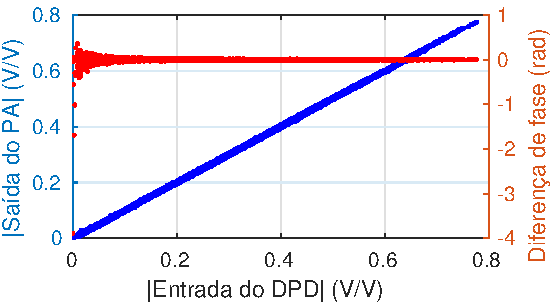
\includegraphics[scale=0.9]{fig2/fig_dpd_ldmos.pdf}
\label{fig:bf-dpd_ldmos}
}\\
\subfloat[GaN{\_}AB{\_}1]{
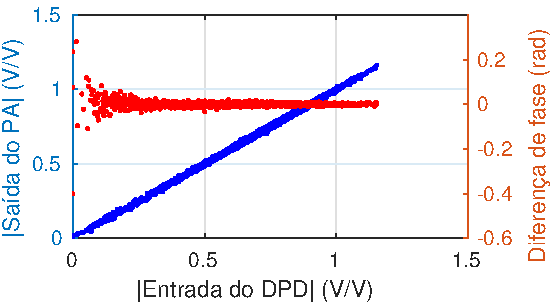
\includegraphics[scale=0.9]{fig2/fig_dpd_sbrt2.pdf}
\label{fig:bf-dpd_sbrt2}
}\\
\subfloat[GaN{\_}AB{\_}2]{
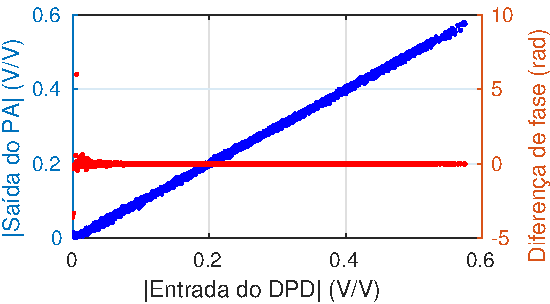
\includegraphics[scale=0.9]{fig2/fig_dpd_tc.pdf}
\label{fig:bf-dpd_tc}
}\\
\subfloat[GaN{\_}Doherty]{
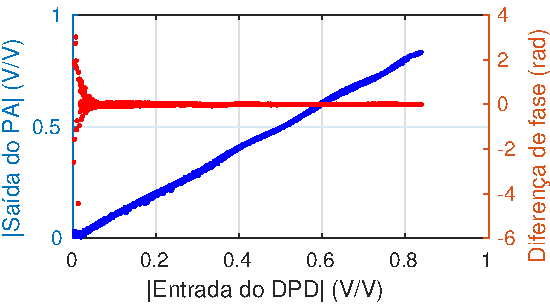
\includegraphics[scale=0.9]{fig2/fig_dpd_doherty.pdf}
\label{fig:bf-dpd_doherty}
}
\caption{Amplitude de saída do PA e diferença de fase na cascata em função da amplitude de entrada do DPD para os diferentes PAs.}
\label{fig:bf-dpd}
\end{figure}


\begin{figure}[H]
\centering
\subfloat[LDMOS{\_}AB]{
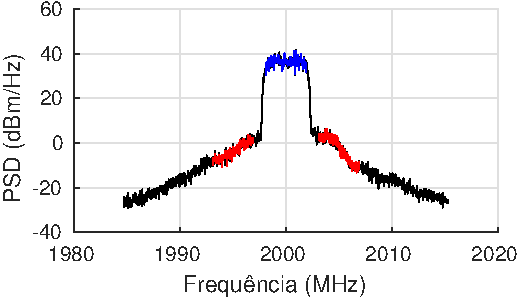
\includegraphics[scale=0.9]{fig2/Frequencia_extraction_ldmos.pdf}
\label{fig:bf-psd_ldmos}
}\\
\subfloat[GaN{\_}AB{\_}1]{
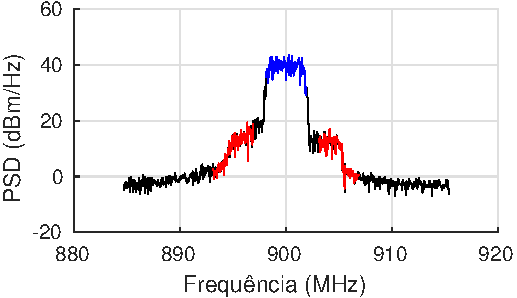
\includegraphics[scale=0.9]{fig2/Frequencia_extraction_sbrt2.pdf}
\label{fig:bf-psd_sbrt2}
}\\
\subfloat[GaN{\_}AB{\_}2]{
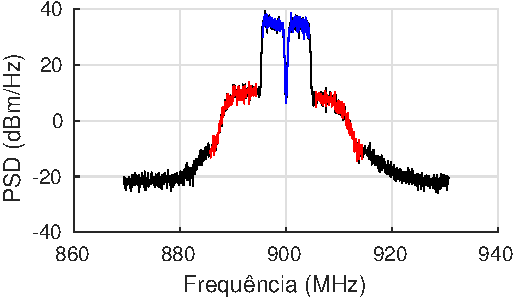
\includegraphics[scale=0.9]{fig2/Frequencia_extraction_tc.pdf}
\label{fig:bf-psd_tc}
}\\
\subfloat[GaN{\_}Doherty]{
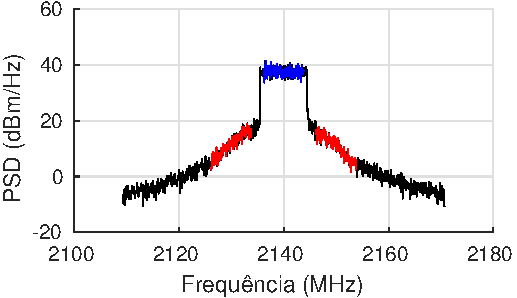
\includegraphics[scale=0.9]{fig2/Frequencia_extraction_doherty.pdf}
\label{fig:bf-psd_doherty}
}\\
\caption{PSD para as entradas estimadas dos DPDs e as saídas medidas dos PAs, considerando-se os conjuntos de dados de treinamento.}
\label{fig:bf-psd}
\end{figure}

 {\setlength{\parindent}{0cm}}


\section{Comparação com a Abordagem Tradicional}

\textcolor{black}{Existindo a necessidade da comparação entre a metodologia tradicional e aquela proposta neste trabalho, um novo estudo de caso deve ser realizado. Este estudo de caso adicional utiliza os dados medidos experimentalmente em um PA linearizado por um DPD já validado pela abordagem tradicional e compara estes resultados com os obtidos por meio da abordagem proposta. Espera-se da abordagem proposta um resultado mais conservador, de modo com que haja a garantia de um rigor na validação do modelo inverso em sua função de DPD.}

{O PA selecionado para o estudo de caso adicional foi um PA GaN classe AB, estimulado por uma portadora em 900 MHz modulada por um sinal WCDMA 3GPP com uma largura de banda de 3,84 MHz e cuja potência média de saída foi de 26 dBm para a extração dos dados. Foram utilizadas 28.800 amostras para o treinamento do modelo e 8.700 amostras para a validação, sendo a frequência de amostragem de 61,44 MHz e as medições realizadas por meio de um VSA Rohde \& Schwarz FSQ \cite{lima2009rfpa}.}

{O modelo de DPD correspondente ao PA foi projetado utilizando-se o modelo polinomial descrito pela seguinte equação:}

\begin{equation}
\tilde{y}(n) = \sum\limits_{p=1}^{P_0} \sum\limits_{m=0}^{M}\tilde{b}_{p,m}|\tilde{x}(n-m)|^{p-1}\tilde{x}(n-m),
\label{dpdcomp}
\end{equation}
{na qual $\tilde{y}(n)$ representa a enésima saída do DPD, $\tilde{x}(n)$ a enésima entrada do DPD, $P_{0}$ a ordem do polinômio resultante, \textit{M} a profundidade de memória requerida pelo polinômio e $\tilde{b}_{p,m}$ é o conjunto de coeficientes que serão ajustados pelo método dos mínimos quadrados de forma a modelar a pré-inversa do PA, sendo definida a ordem do polinômio resultante $P_{0}$ como 7 e a profundidade de memória \textit{M} como 3.}

{Dois conjuntos de dados diferentes foram utilizados para esta comparação. O primeiro deles é formado pelos valores de entrada e saída da cascata e foi utilizado para a obtenção dos valores de NMSE e ACPR referentes a validação tradicional, assim como para a obtenção da \autoref{abr_trad}. Em outras palavras, para a obtenção deste primeiro conjunto de dados, uma nova medição do PA foi realizada após o treinamento do DPD, no qual um sinal conhecido foi primeiramente aplicado na entrada do DPD e a sequência pré-distorcida gerada pelo DPD foi então aplicada na entrada do PA. O segundo conjunto de dados é formado pelos valores de entrada e saída do PA medidos antes da identificação do DPD e foi utilizado para a obtenção dos valores de NMSE e ACPR referentes ao método proposto de validação e também para a obtenção da \autoref{abr_prp}.}

{O cálculo do ACPR foi realizado para os sinais de entrada e saída das cascatas. Foi utilizada uma diferença entre a frequência central da faixa central e as frequências centrais das faixas adjacentes de 5 MHz.}

{Na Tabela \ref{nmse_comp} são comparados os valores de NMSE e ACPR. Verifica-se através da análise do NMSE que o resultado da metodologia proposta apresenta uma estimativa mais conservadora em relação à realidade, uma consequência do erro adicional ao sistema pela resolução do problema inverso. Pela Tabela \ref{nmse_comp}, verifica-se que os valores de ACPR obtidos na entrada e saída da cascata que valida o DPD usando a estratégia proposta são mais próximos entre si do que os respectivos valores para a cascata que valida o DPD usando a estratégia tradicional. Em específico, na cascata que valida o DPD por meio da estratégia proposta, as diferenças de ACPR de entrada e saída são de no máximo 4,0 dB, enquanto que na cascata que valida o DPD por meio da estratégia tradicional, as diferenças de ACPR de entrada e saída são de até 21,5 dB. Cumpre ressaltar que, na estratégia tradicional, busca-se estimar valores extremamente baixos de ACPR, o que de fato configura-se em uma tarefa muito difícil de ser cumprida. Dessa forma, pode-se concluir que, em ambas as estratégias tradicional e proposta, o objetivo de obter um sinal de saída da cascata que é uma réplica do sinal de entrada da cascata é cumprido de maneira bastante satisfatória.}

\begin{table}[!tbh]
\centering
\caption{Valores de NMSE e ACPR para a comparação entre as duas abordagens.}
\begin{tabular}{|c|c|c|}
\hline 
\textbf{Abordagem} & \textbf{Tradicional} & \textbf{Proposta}\\ 
\hline 
NMSE (dB) & -44,6 & -38,9 \\
\hline
$ACPR_{sup}$ de Entrada (dB) & -77,2 & -36,0 \\ 
\hline 
$ACPR_{inf}$ de Entrada (dB) & -77,8 & -33,6 \\ 
\hline 
$ACPR_{sup}$ de Saída (dB) & -57,9 & -39,1 \\ 
\hline 
$ACPR_{inf}$ de Saída (dB) & -56,3 & -37,6 \\ 
\hline 
\end{tabular}
\label{nmse_comp}
\end{table}

{Na \autoref{abr_txp} são observados tanto o comportamento linear necessário como a pequena diferença de fase, condições necessárias para o bom funcionamento do DPD.}

\begin{figure}[H]
\centering
\subfloat[Tradicional]{
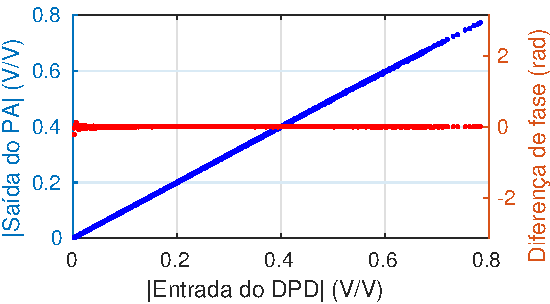
\includegraphics[scale=0.9]{fig2/fig_dpd_trad.pdf}
\label{abr_trad}
}\\
\subfloat[Proposto]{
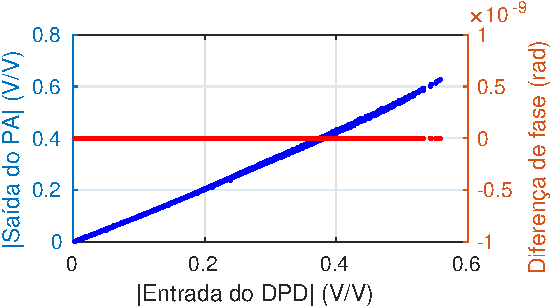
\includegraphics[scale=0.9]{fig2/fig_dpd_new.pdf}
\label{abr_prp}
}
\caption{Amplitude de saída do PA e diferença de fase na cascata em função da amplitude de entrada do DPD para: a) Método tradicional de validação; b) Método proposto de validação}
\label{abr_txp}
\end{figure}



% ELEMENTOS PÓS-TEXTUAIS
% ----------------------------------------------------------
\postextual

% Ajuste vertical do titulo de referencias no sumário
% ----------------------------------------------------------
\addtocontents{toc}{\vspace{-24pt}}

% Referências bibliográficas
% ----------------------------------------------------------
%\bibliography{referencias}

\printbibliography[heading=bay]
% ----------------------------------------------------------

% Ajuste vertical dos titulos dos capitulos postextuais
% ----------------------------------------------------------
\addtocontents{toc}{\vspace{-12pt}}

% Glossário
% ----------------------------------------------------------
% Consulte o manual da classe abntex2 para orientações sobre o glossário.
%
%\glossary

% Apêndices
% ----------------------------------------------------------
\ifthenelse{\equal{\terApendice}{Sim}}
{\begin{apendicesenv}

        % Numeração arábica para os apêndices
        % --------------------------------------------------
        \renewcommand{\thechapter}{\arabic{chapter}}
        % Imprime uma página indicando o início dos apêndices
        % \partapendices

        % Existem várias formas de se colocar anexos.
        % O exemplo abaixo coloca 2 apêndices denominados de 
        % DESENVOLVIMENTO DETALHADO DA PINTURA e 
        % ESCOLHA DO MATERIAL DE IMPRESSÃO:
        % ---
        % --- insere um capítulo que é tratado como um apêndice
        %\chapter{DESENVOLVIMENTO DETALHADO DA PINTURA}
        % 
        %\lipsum[29] % gera um parágrafo
        %
        % --- insere um capítulo que é tratado como um apêndice
        %\chapter{ESCOLHA DO MATERIAL DE IMPRESSÃO}
        % 
        %\lipsum[30] % gera um parágrafo

        % --- Insere o texto do arquivo ap01.tex
        % 
        % --- O conteúdo do arquivo pode ser vários anexos ou um único apêndices.
        %     A vantagem de se utilizar este procedimento é de suprimi-lo
        %     das compilações enquanto se processa o resto do documento.

           % --- insere um capítulo que é tratado como um apêndice
   \poschap{ESCOLHA DO MATERIAL - colocado no apendice}
    
   \lipsum[30] % gera um parágrafo
   \section*{Testes se\c{C}\~aO}

    \lipsum[22] % gera um parágrafo
	
	\poschap{ESCOLHA DO MATERIAL DE IMPRESSÃO- colocado no apendice}
    \lipsum[32] % gera um parágrafo

\end{apendicesenv}
}{}


% Anexos
% ----------------------------------------------------------
\ifthenelse{\equal{\terAnexo}{Sim}}{
\begin{anexosenv}

        % Numeração arábica para os apêndices
        % --------------------------------------------------
        \renewcommand{\thechapter}{\arabic{chapter}}
        % --- Imprime uma página indicando o início dos anexos
        % \partanexos

        % Existem várias formas de se colocar anexos.
        % O exemplo abaixo coloca 2 anexos denominados de 
        % TABELA DE VALORES e GRÁFICOS DE BALANCEMANTO:
        % ---
        % --- insere um capítulo que é tratado como um anexo
        %\chapter{TABELAS DE VALORES}
        % 
        %\lipsum[31] % gera um parágrafo
        %
        % --- insere um capítulo que é tratado como um anexo
        %\chapter{GRÁFICOS DE BALANCEAMENTO}
        % 
        %\lipsum[32] % gera um parágrafo

        % --- Insere o texto do arquivo ax01.tex
        % 
        % --- O conteúdo do arquivo pode ser vários anexos ou um único anexo.
        %     A vantagem de se utilizar este procedimento é de suprimi-lo
        %     das compilações enquanto se processa o resto do documento.

            % --- insere um capítulo que é tratado como um apêndice
   \chapter{anexando ESCOLHA DO MATERIAL}
    
   \lipsum[30] % gera um parágrafo
    \section*{anexando testes secao}
    

\chapter{anexando ESCOLHA DO MATERIAL DE IMPRESSÃO}
    
   \lipsum[32] % gera um parágrafo 
\end{anexosenv}
}{}

% INDICE REMISSIVO
%---------------------------------------------------------------------
\ifthenelse{\equal{\terIndiceR}{Sim}}{
\phantompart
\printindex
}{}

\end{document}
